%%
% Copyright (c) 2017 - 2025, Pascal Wagler;
% Copyright (c) 2014 - 2025, John MacFarlane
%
% All rights reserved.
%
% Redistribution and use in source and binary forms, with or without
% modification, are permitted provided that the following conditions
% are met:
%
% - Redistributions of source code must retain the above copyright
% notice, this list of conditions and the following disclaimer.
%
% - Redistributions in binary form must reproduce the above copyright
% notice, this list of conditions and the following disclaimer in the
% documentation and/or other materials provided with the distribution.
%
% - Neither the name of John MacFarlane nor the names of other
% contributors may be used to endorse or promote products derived
% from this software without specific prior written permission.
%
% THIS SOFTWARE IS PROVIDED BY THE COPYRIGHT HOLDERS AND CONTRIBUTORS
% "AS IS" AND ANY EXPRESS OR IMPLIED WARRANTIES, INCLUDING, BUT NOT
% LIMITED TO, THE IMPLIED WARRANTIES OF MERCHANTABILITY AND FITNESS
% FOR A PARTICULAR PURPOSE ARE DISCLAIMED. IN NO EVENT SHALL THE
% COPYRIGHT OWNER OR CONTRIBUTORS BE LIABLE FOR ANY DIRECT, INDIRECT,
% INCIDENTAL, SPECIAL, EXEMPLARY, OR CONSEQUENTIAL DAMAGES (INCLUDING,
% BUT NOT LIMITED TO, PROCUREMENT OF SUBSTITUTE GOODS OR SERVICES;
% LOSS OF USE, DATA, OR PROFITS; OR BUSINESS INTERRUPTION) HOWEVER
% CAUSED AND ON ANY THEORY OF LIABILITY, WHETHER IN CONTRACT, STRICT
% LIABILITY, OR TORT (INCLUDING NEGLIGENCE OR OTHERWISE) ARISING IN
% ANY WAY OUT OF THE USE OF THIS SOFTWARE, EVEN IF ADVISED OF THE
% POSSIBILITY OF SUCH DAMAGE.
%%

%%
% This is the Eisvogel pandoc LaTeX template.
%
% For usage information and examples visit the official GitHub page:
% https://github.com/Wandmalfarbe/pandoc-latex-template
%%
% Options for packages loaded elsewhere
\PassOptionsToPackage{unicode}{hyperref}
\PassOptionsToPackage{hyphens}{url}
\PassOptionsToPackage{dvipsnames,svgnames,x11names,table}{xcolor}
\documentclass[
  american,
  11pt,
  letterpaper,
  oneside  ,captions=tableheading
]{scrartcl}
\usepackage{xcolor}
\usepackage[margin=1in]{geometry}
\usepackage{amsmath,amssymb}

% add backlinks to footnote references, cf. https://tex.stackexchange.com/questions/302266/make-footnote-clickable-both-ways
\usepackage{footnotebackref}
\setcounter{secnumdepth}{5}
\usepackage{iftex}
\ifPDFTeX
  \usepackage[T1]{fontenc}
  \usepackage[utf8]{inputenc}
  \usepackage{textcomp} % provide euro and other symbols
\else % if luatex or xetex
  \usepackage{unicode-math} % this also loads fontspec
  \defaultfontfeatures{Scale=MatchLowercase}
  \defaultfontfeatures[\rmfamily]{Ligatures=TeX,Scale=1}
\fi
\usepackage{lmodern}
\ifPDFTeX\else
  % xetex/luatex font selection
  \setmainfont[]{DejaVu Serif}
  \setsansfont[]{DejaVu Sans}
  \setmonofont[]{DejaVu Sans Mono}
\fi
% Use upquote if available, for straight quotes in verbatim environments
\IfFileExists{upquote.sty}{\usepackage{upquote}}{}
\IfFileExists{microtype.sty}{% use microtype if available
  \usepackage[]{microtype}
  \UseMicrotypeSet[protrusion]{basicmath} % disable protrusion for tt fonts
}{}

\usepackage{setspace}
\makeatletter
\@ifundefined{KOMAClassName}{% if non-KOMA class
  \IfFileExists{parskip.sty}{%
    \usepackage{parskip}
  }{% else
    \setlength{\parindent}{0pt}
    \setlength{\parskip}{6pt plus 2pt minus 1pt}}
}{% if KOMA class
  \KOMAoptions{parskip=half}}
\makeatother
\usepackage{listings}
\newcommand{\passthrough}[1]{#1}
\lstset{defaultdialect=[5.3]Lua}
\lstset{defaultdialect=[x86masm]Assembler}
\usepackage{etoolbox}
\BeforeBeginEnvironment{lstlisting}{\par\noindent\begin{minipage}{\linewidth}}
\AfterEndEnvironment{lstlisting}{\end{minipage}\par\addvspace{\topskip}}
\usepackage{longtable,booktabs,array}
\newcounter{none} % for unnumbered tables
\usepackage{calc} % for calculating minipage widths
% Correct order of tables after \paragraph or \subparagraph
\usepackage{etoolbox}
\makeatletter
\patchcmd\longtable{\par}{\if@noskipsec\mbox{}\fi\par}{}{}
\makeatother
% Allow footnotes in longtable head/foot
\IfFileExists{footnotehyper.sty}{\usepackage{footnotehyper}}{\usepackage{footnote}}
\makesavenoteenv{longtable}
\ifLuaTeX
\usepackage[bidi=basic,shorthands=off]{babel}
\else
\usepackage[bidi=default,shorthands=off]{babel}
\fi
\ifPDFTeX
\else
\babelfont{rm}[]{DejaVu Serif}
\fi
\ifLuaTeX
  \usepackage{selnolig} % disable illegal ligatures
\fi
\setlength{\emergencystretch}{3em} % prevent overfull lines
\providecommand{\tightlist}{%
  \setlength{\itemsep}{0pt}\setlength{\parskip}{0pt}}
\usepackage{graphicx}
\usepackage{xurl}
\usepackage{rotating}
\usepackage{booktabs}
\usepackage{bookmark}
\IfFileExists{xurl.sty}{\usepackage{xurl}}{} % add URL line breaks if available
\urlstyle{same}
\definecolor{default-linkcolor}{HTML}{A50000}
\definecolor{default-filecolor}{HTML}{A50000}
\definecolor{default-citecolor}{HTML}{4077C0}
\definecolor{default-urlcolor}{HTML}{4077C0}

\hypersetup{
  pdftitle={Natural Language to SQL in Healthcare: Bridging Analytics Maturity Gaps, Workforce Turnover, and Technical Barriers Through Conversational AI Platforms},
  pdfauthor={Samuel T Harrold, Yuimedi},
  pdflang={en-US},
  pdfkeywords={healthcare analytics, natural language processing, SQL
generation, institutional memory, conversational AI, healthcare
informatics, workforce turnover, analytics maturity},
  colorlinks=true,
  linkcolor={blue},
  filecolor={default-filecolor},
  citecolor={blue},
  urlcolor={blue},
  breaklinks=true,
  pdfcreator={LaTeX via pandoc with the Eisvogel template}}

\title{Natural Language to SQL in Healthcare: Bridging Analytics
Maturity Gaps, Workforce Turnover, and Technical Barriers Through
Conversational AI Platforms}
\author{Samuel T Harrold, Yuimedi}
\date{December 2025}


%
% for the background color of the title page
%
\usepackage{pagecolor}
\usepackage{afterpage}

%
% break urls
%
\PassOptionsToPackage{hyphens}{url}

%
% When using babel or polyglossia with biblatex, loading csquotes is recommended
% to ensure that quoted texts are typeset according to the rules of your main language.
%
\usepackage{csquotes}

%
% captions
%
\definecolor{caption-color}{HTML}{777777}
\usepackage[font={stretch=1.2}, textfont={color=caption-color}, position=top, skip=4mm, labelfont=bf, singlelinecheck=false, justification=raggedright]{caption}
\setcapindent{0em}

%
% blockquote
%
\definecolor{blockquote-border}{RGB}{221,221,221}
\definecolor{blockquote-text}{RGB}{119,119,119}
\usepackage{mdframed}
\newmdenv[rightline=false,bottomline=false,topline=false,linewidth=3pt,linecolor=blockquote-border,skipabove=\parskip]{customblockquote}
\renewenvironment{quote}{\begin{customblockquote}\list{}{\rightmargin=0em\leftmargin=0em}%
\item\relax\color{blockquote-text}\ignorespaces}{\unskip\unskip\endlist\end{customblockquote}}

%
% Source Sans Pro as the default font family
% Source Code Pro for monospace text
%
% 'default' option sets the default
% font family to Source Sans Pro, not \sfdefault.
%
% Note that the font has been officially renamed to `Source Sans 3`, and
% the version provided by the `sourcesanspro` package is slightly outdated.
% You can install the newer version locally and use it, for example, with
% `mainfont: "Source Sans 3"` in the YAML metadata (requires XeTeX or LuaTeX).
%
\ifnum 0\ifxetex 1\fi\ifluatex 1\fi=0 % if pdftex
    \usepackage[default]{sourcesanspro}
  \usepackage{sourcecodepro}
  \else % if not pdftex
    \fi

%
% heading color
%
\definecolor{heading-color}{RGB}{40,40,40}
% By default, the KOMA-Script classes will typeset sectioning headings in
% sans-serif. Use the normal body font for headings.
\addtokomafont{disposition}{\normalfont\color{heading-color}\bfseries}

%
% variables for title, author and date
%
\usepackage{titling}
\title{Natural Language to SQL in Healthcare: Bridging Analytics
Maturity Gaps, Workforce Turnover, and Technical Barriers Through
Conversational AI Platforms}
\author{Samuel T Harrold, Yuimedi}
\date{December 2025}

%
% tables
%

\definecolor{table-row-color}{HTML}{F5F5F5}
\definecolor{table-rule-color}{HTML}{999999}

%\arrayrulecolor{black!40}
\arrayrulecolor{table-rule-color}     % color of \toprule, \midrule, \bottomrule
\setlength\heavyrulewidth{0.3ex}      % thickness of \toprule, \bottomrule
\renewcommand{\arraystretch}{1.3}     % spacing (padding)


%
% remove paragraph indentation
%
\setlength{\parindent}{0pt}
\setlength{\parskip}{6pt plus 2pt minus 1pt}
\setlength{\emergencystretch}{3em}  % prevent overfull lines

%
%
% Listings
%
%


%
% general listing colors
%
\definecolor{listing-background}{HTML}{F7F7F7}
\definecolor{listing-rule}{HTML}{B3B2B3}
\definecolor{listing-numbers}{HTML}{B3B2B3}
\definecolor{listing-text-color}{HTML}{000000}
\definecolor{listing-keyword}{HTML}{435489}
\definecolor{listing-keyword-2}{HTML}{1284CA} % additional keywords
\definecolor{listing-keyword-3}{HTML}{9137CB} % additional keywords
\definecolor{listing-identifier}{HTML}{435489}
\definecolor{listing-string}{HTML}{00999A}
\definecolor{listing-comment}{HTML}{8E8E8E}

\lstdefinestyle{eisvogel_listing_style}{
  language         = java,
  numbers          = left,
  xleftmargin      = 2.7em,
  framexleftmargin = 2.5em,
  backgroundcolor  = \color{listing-background},
  basicstyle       = \color{listing-text-color}\linespread{1.0}%
                      \lst@ifdisplaystyle%
                      \small%
                      \fi\ttfamily{},
  breaklines       = true,
  frame            = single,
  framesep         = 0.19em,
  rulecolor        = \color{listing-rule},
  frameround       = ffff,
  tabsize          = 4,
  numberstyle      = \color{listing-numbers},
  aboveskip        = 1.0em,
  belowskip        = 0.1em,
  abovecaptionskip = 0em,
  belowcaptionskip = 1.0em,
  keywordstyle     = {\color{listing-keyword}\bfseries},
  keywordstyle     = {[2]\color{listing-keyword-2}\bfseries},
  keywordstyle     = {[3]\color{listing-keyword-3}\bfseries\itshape},
  sensitive        = true,
  identifierstyle  = \color{listing-identifier},
  commentstyle     = \color{listing-comment},
  stringstyle      = \color{listing-string},
  showstringspaces = false,
  escapeinside     = {/*@}{@*/}, % Allow LaTeX inside these special comments
  literate         =
  {á}{{\'a}}1 {é}{{\'e}}1 {í}{{\'i}}1 {ó}{{\'o}}1 {ú}{{\'u}}1
  {Á}{{\'A}}1 {É}{{\'E}}1 {Í}{{\'I}}1 {Ó}{{\'O}}1 {Ú}{{\'U}}1
  {à}{{\`a}}1 {è}{{\`e}}1 {ì}{{\`i}}1 {ò}{{\`o}}1 {ù}{{\`u}}1
  {À}{{\`A}}1 {È}{{\`E}}1 {Ì}{{\`I}}1 {Ò}{{\`O}}1 {Ù}{{\`U}}1
  {ä}{{\"a}}1 {ë}{{\"e}}1 {ï}{{\"i}}1 {ö}{{\"o}}1 {ü}{{\"u}}1
  {Ä}{{\"A}}1 {Ë}{{\"E}}1 {Ï}{{\"I}}1 {Ö}{{\"O}}1 {Ü}{{\"U}}1
  {â}{{\^a}}1 {ê}{{\^e}}1 {î}{{\^i}}1 {ô}{{\^o}}1 {û}{{\^u}}1
  {Â}{{\^A}}1 {Ê}{{\^E}}1 {Î}{{\^I}}1 {Ô}{{\^O}}1 {Û}{{\^U}}1
  {œ}{{\oe}}1 {Œ}{{\OE}}1 {æ}{{\ae}}1 {Æ}{{\AE}}1 {ß}{{\ss}}1
  {ç}{{\c c}}1 {Ç}{{\c C}}1 {ø}{{\o}}1 {å}{{\r a}}1 {Å}{{\r A}}1
  {€}{{\EUR}}1 {£}{{\pounds}}1 {«}{{\guillemotleft}}1
  {»}{{\guillemotright}}1 {ñ}{{\~n}}1 {Ñ}{{\~N}}1 {¿}{{?`}}1
  {…}{{\ldots}}1 {≥}{{>=}}1 {≤}{{<=}}1 {„}{{\glqq}}1 {“}{{\grqq}}1
  {”}{{''}}1
}
\lstset{style=eisvogel_listing_style}

%
% Java (Java SE 12, 2019-06-22)
%
\lstdefinelanguage{Java}{
  morekeywords={
    % normal keywords (without data types)
    abstract,assert,break,case,catch,class,continue,default,
    do,else,enum,exports,extends,final,finally,for,if,implements,
    import,instanceof,interface,module,native,new,package,private,
    protected,public,requires,return,static,strictfp,super,switch,
    synchronized,this,throw,throws,transient,try,volatile,while,
    % var is an identifier
    var
  },
  morekeywords={[2] % data types
    % primitive data types
    boolean,byte,char,double,float,int,long,short,
    % String
    String,
    % primitive wrapper types
    Boolean,Byte,Character,Double,Float,Integer,Long,Short
    % number types
    Number,AtomicInteger,AtomicLong,BigDecimal,BigInteger,DoubleAccumulator,DoubleAdder,LongAccumulator,LongAdder,Short,
    % other
    Object,Void,void
  },
  morekeywords={[3] % literals
    % reserved words for literal values
    null,true,false,
  },
  sensitive,
  morecomment  = [l]//,
  morecomment  = [s]{/*}{*/},
  morecomment  = [s]{/**}{*/},
  morestring   = [b]",
  morestring   = [b]',
}

\lstdefinelanguage{XML}{
  morestring      = [b]",
  moredelim       = [s][\bfseries\color{listing-keyword}]{<}{\ },
  moredelim       = [s][\bfseries\color{listing-keyword}]{</}{>},
  moredelim       = [l][\bfseries\color{listing-keyword}]{/>},
  moredelim       = [l][\bfseries\color{listing-keyword}]{>},
  morecomment     = [s]{<?}{?>},
  morecomment     = [s]{<!--}{-->},
  commentstyle    = \color{listing-comment},
  stringstyle     = \color{listing-string},
  identifierstyle = \color{listing-identifier}
}

%
% header and footer
%
\usepackage[headsepline,footsepline]{scrlayer-scrpage}

\newpairofpagestyles{eisvogel-header-footer}{
  \clearpairofpagestyles
  \ihead*{NL2SQL in Healthcare}
  \chead*{}
  \ohead*{December 2025}
  \ifoot*{\hspace{0pt}}
  \cfoot*{\thepage}
  \ofoot*{\hspace{0pt}}
  \addtokomafont{pageheadfoot}{\upshape}
}
\pagestyle{eisvogel-header-footer}



%
% Define watermark
%

\begin{document}

\begin{titlepage}
\newgeometry{left=6cm}
\definecolor{titlepage-color}{HTML}{FFFFFF}
\newpagecolor{titlepage-color}\afterpage{\restorepagecolor}
\newcommand{\colorRule}[3][black]{\textcolor[HTML]{#1}{\rule{#2}{#3}}}
\begin{flushleft}
\noindent
\\[-1em]
\color[HTML]{000000}
\makebox[0pt][l]{\colorRule[000000]{1.3\textwidth}{2pt}}
\par
\noindent

{
  \setstretch{1.4}
  \vfill
  \noindent {\huge \textbf{\textsf{Natural Language to SQL in
Healthcare: Bridging Analytics Maturity Gaps, Workforce Turnover, and
Technical Barriers Through Conversational AI Platforms}}}
    \vskip 2em
  \noindent {\Large \textsf{Samuel T Harrold, Yuimedi}}
  \vfill
}


\textsf{December 2025}
\end{flushleft}
\end{titlepage}
\restoregeometry
\pagenumbering{arabic}

% don't generate the default title
% \maketitle
\begin{abstract}
This research examines the evidence for implementing conversational AI
platforms in healthcare analytics, addressing three critical challenges:
low healthcare analytics maturity, workforce turnover with institutional
memory loss, and technical barriers in natural language to SQL
generation. Through review of peer-reviewed benchmarking studies and
industry implementations, we demonstrate that natural language
interfaces can democratize analytics access while preserving
institutional knowledge. Healthcare-specific text-to-SQL benchmarks show
significant progress, though current models are ``not yet sufficiently
accurate for unsupervised use'' in clinical settings. Healthcare IT
staff turnover of \textasciitilde34\% (as of 2004), the highest among IT
sectors at that time, creates institutional memory loss, while low-code
implementations demonstrate significant efficiency gains and cost
savings. The convergence of technical advances in NL2SQL generation,
analytics maturity challenges in healthcare organizations, and workforce
turnover creates conditions warranting organizational assessment of
conversational AI platforms with appropriate governance. This paper
contributes a three-pillar analytical framework (analytics maturity,
workforce turnover, technical barriers) and positions healthcare
conversational AI as a knowledge portal architecture for institutional
memory preservation.
\end{abstract}


{
\setcounter{tocdepth}{3}
\tableofcontents
}
\setstretch{1.15}
\section{Introduction}\label{introduction}

\subsection{Background}\label{background}

Healthcare analytics has emerged as a critical capability for improving
patient outcomes, reducing costs, and enhancing operational efficiency.
While healthcare organizations must balance cost management, regulatory
compliance, and operational efficiency, these concerns serve a primary
institutional imperative: delivering high-quality patient care.
Analytics initiatives that fail to advance this core mission, or worse,
that divert resources and attention without improving care delivery,
represent a misalignment with healthcare's fundamental purpose.

However, the sector faces unique challenges that distinguish it from
other data-intensive industries. Unlike technology or financial
services, healthcare combines complex clinical workflows, extensive
regulatory requirements, and a workforce with limited technical training
but deep domain expertise {[}I11{]}.

The Healthcare Information Management Systems Society (HIMSS) Analytics
Maturity Assessment Model (AMAM) provides the industry standard for
measuring healthcare analytics capabilities across seven stages, from
basic data collection to advanced predictive modeling and AI
integration. Recent assessments reveal a sobering reality: as of 2024,
only 26 organizations worldwide have achieved Stage 6 maturity, with
merely 13 reaching Stage 7, the highest level characterized by
predictive analytics and AI integration {[}I1{]}.

This analytics maturity crisis occurs amid accelerating technological
advances in natural language processing and conversational AI. Large
language models have demonstrated remarkable capabilities in
understanding clinical terminology, generating SQL queries, and bridging
the gap between natural language questions and structured data analysis.
These developments create unprecedented opportunities to democratize
healthcare analytics access.

Simultaneously, healthcare faces an institutional memory crisis driven
by workforce turnover rates significantly higher than other
knowledge-intensive sectors. A 2004 study found healthcare IT staff
turnover of 34\% {[}A10{]}, the highest rate among all IT organization
types studied at that time, creating cascading knowledge loss,
particularly in analytics roles where expertise combines domain
knowledge with technical skills. Traditional knowledge management
approaches prove inadequate for preserving the tacit knowledge essential
for effective healthcare data analysis.

\subsection{Problem Statement}\label{problem-statement}

Healthcare organizations face three critical, interconnected challenges
that collectively threaten their ability to become data-driven
enterprises:

\subsubsection{Low Healthcare Analytics
Maturity}\label{low-healthcare-analytics-maturity}

Despite massive investments in electronic health records and data
infrastructure, healthcare organizations struggle to advance beyond
basic reporting capabilities. The HIMSS AMAM reveals that most
organizations remain at Stages 0-3, characterized by fragmented data
sources, limited automated reporting, and minimal predictive
capabilities {[}I1{]}. This low maturity severely constrains
evidence-based decision making and operational optimization.

\subsubsection{Technical Barriers to Data
Access}\label{technical-barriers-to-data-access}

Healthcare professionals possess deep clinical knowledge but lack the
technical skills required for data analysis. Traditional analytics tools
require SQL expertise, statistical knowledge, and familiarity with
complex database schemas, capabilities that clinical staff often do not
possess nor have time to develop. This creates a fundamental disconnect
between those who understand the clinical questions and those who can
access the data to answer them {[}A14{]}, {[}A15{]}, {[}A16{]}. Drawing
on principles from code modernization, AI-assisted interfaces can bridge
this gap by transforming legacy technical requirements into natural
language interactions {[}I8{]}. Foundational research on natural
language interfaces to databases established that modular architecture
principles enable effective bridging of legacy data access challenges
{[}A46{]}, with modern implementations demonstrating that the same large
language models underlying code modernization can serve as natural
language interfaces to legacy systems {[}A47{]}, {[}A48{]}.

\subsubsection{Institutional Memory Loss from Workforce
Turnover}\label{institutional-memory-loss-from-workforce-turnover}

A 2004 study found healthcare IT staff experienced the highest turnover
among IT sectors at 34\% annually (calculated as 1/2.9 years average
tenure), with average tenure of only 2.9 years, the lowest among IT
sectors studied at that time {[}A10{]}. This creates significant
institutional memory loss. When experienced analysts, clinical
informatics professionals, or data-savvy clinicians leave, they take
with them irreplaceable knowledge about data definitions, business
rules, analytical approaches, and organizational context. This knowledge
proves extremely difficult to document and transfer through traditional
means.

The implications are measurable in operational terms and patient care
quality. Organizations continue investing in analytics infrastructure
while struggling to realize value from their data assets. Empirical
research demonstrates that a 10-percentage-point increase in nursing
staff turnover is associated with 0.241 additional health inspection
citations and decreased assessment-based quality measures {[}A62{]}.
When analytics barriers are addressed, outcomes improve substantially:
one Medicare ACO reduced readmission rates from 24\% to 17.8\% and
achieved \$1.6 million in cost savings by implementing data analytics to
overcome EHR fragmentation {[}A64{]}. Technical barriers remain
pervasive, with 68\% of healthcare organizations citing data
interoperability as the leading obstacle to analytics adoption, followed
by privacy concerns (64\%) and insufficient staff training (59\%)
{[}A65{]}. Physician technology adoption faces empirically validated
barriers including perceived threat and inequity from workflow changes,
directly impacting behavioral intentions toward analytics tools
{[}A63{]}. These three interconnected challenges represent operational
inefficiencies with demonstrated implications for healthcare delivery.

\subsection{Objectives}\label{objectives}

This research aims to provide evidence-based guidance for healthcare
organizations seeking to address these interconnected challenges through
conversational AI platforms. Specific objectives include:

\subsubsection{Primary Objective}\label{primary-objective}

Demonstrate through systematic literature review that conversational AI
platforms represent an evidence-based solution to healthcare's analytics
challenges, with empirical validation of their effectiveness in
addressing analytics maturity, technical barriers, and institutional
memory preservation.

\subsubsection{Secondary Objectives}\label{secondary-objectives}

\begin{enumerate}
\def\labelenumi{\arabic{enumi}.}
\tightlist
\item
  \textbf{Synthesize current evidence} on natural language to SQL
  generation capabilities and limitations in healthcare contexts
\item
  \textbf{Document the extent} of analytics maturity challenges across
  healthcare organizations globally
\item
  \textbf{Quantify the impact} of workforce turnover on institutional
  memory and analytics capabilities
\item
  \textbf{Identify implementation strategies} supported by empirical
  evidence from early adopters
\item
  \textbf{Establish ROI evidence} for conversational AI platform
  investments in healthcare settings
\end{enumerate}

\subsubsection{Non-Goals}\label{non-goals}

This research explicitly does not address:

\begin{itemize}
\tightlist
\item
  Specific vendor comparisons or product recommendations
\item
  Implementation details for particular healthcare IT environments
\item
  Regulatory compliance strategies for specific jurisdictions
\item
  Technical architecture specifications for conversational AI systems
\end{itemize}

Note: Analysis of market dynamics and structural factors explaining why
institution-specific analytics challenges persist is within scope. This
market-level analysis provides necessary context for evaluating solution
approaches and differs from product comparison, which would evaluate
specific vendor offerings against each other or recommend particular
products.

\subsection{Contributions}\label{contributions}

This paper makes three contributions to the healthcare informatics
literature:

\begin{enumerate}
\def\labelenumi{\arabic{enumi}.}
\item
  \textbf{Three-Pillar Analytical Framework}: We synthesize evidence
  from three previously disconnected research domains (healthcare
  analytics maturity, workforce turnover, and natural language
  processing) into a unified analytical framework that reveals how these
  challenges interconnect and compound each other: low maturity
  accelerates turnover, turnover degrades maturity, and technical
  barriers prevent recovery from either.
\item
  \textbf{Healthcare Knowledge Portal Architecture}: Drawing on
  established knowledge management literature {[}A25, A26{]}, we
  position conversational AI platforms as healthcare knowledge portals,
  which are systems that provide mechanisms for knowledge acquisition,
  storage, sharing, and utilization. This framing addresses the
  institutional memory crisis in healthcare by embedding organizational
  expertise within AI systems rather than relying on individual staff
  retention. Figure 1 illustrates this architecture, showing how
  clinical users interact with a conversational AI interface that draws
  on organizational knowledge infrastructure to generate contextual
  insights.
\end{enumerate}

\begin{figure}[htbp]
\centering
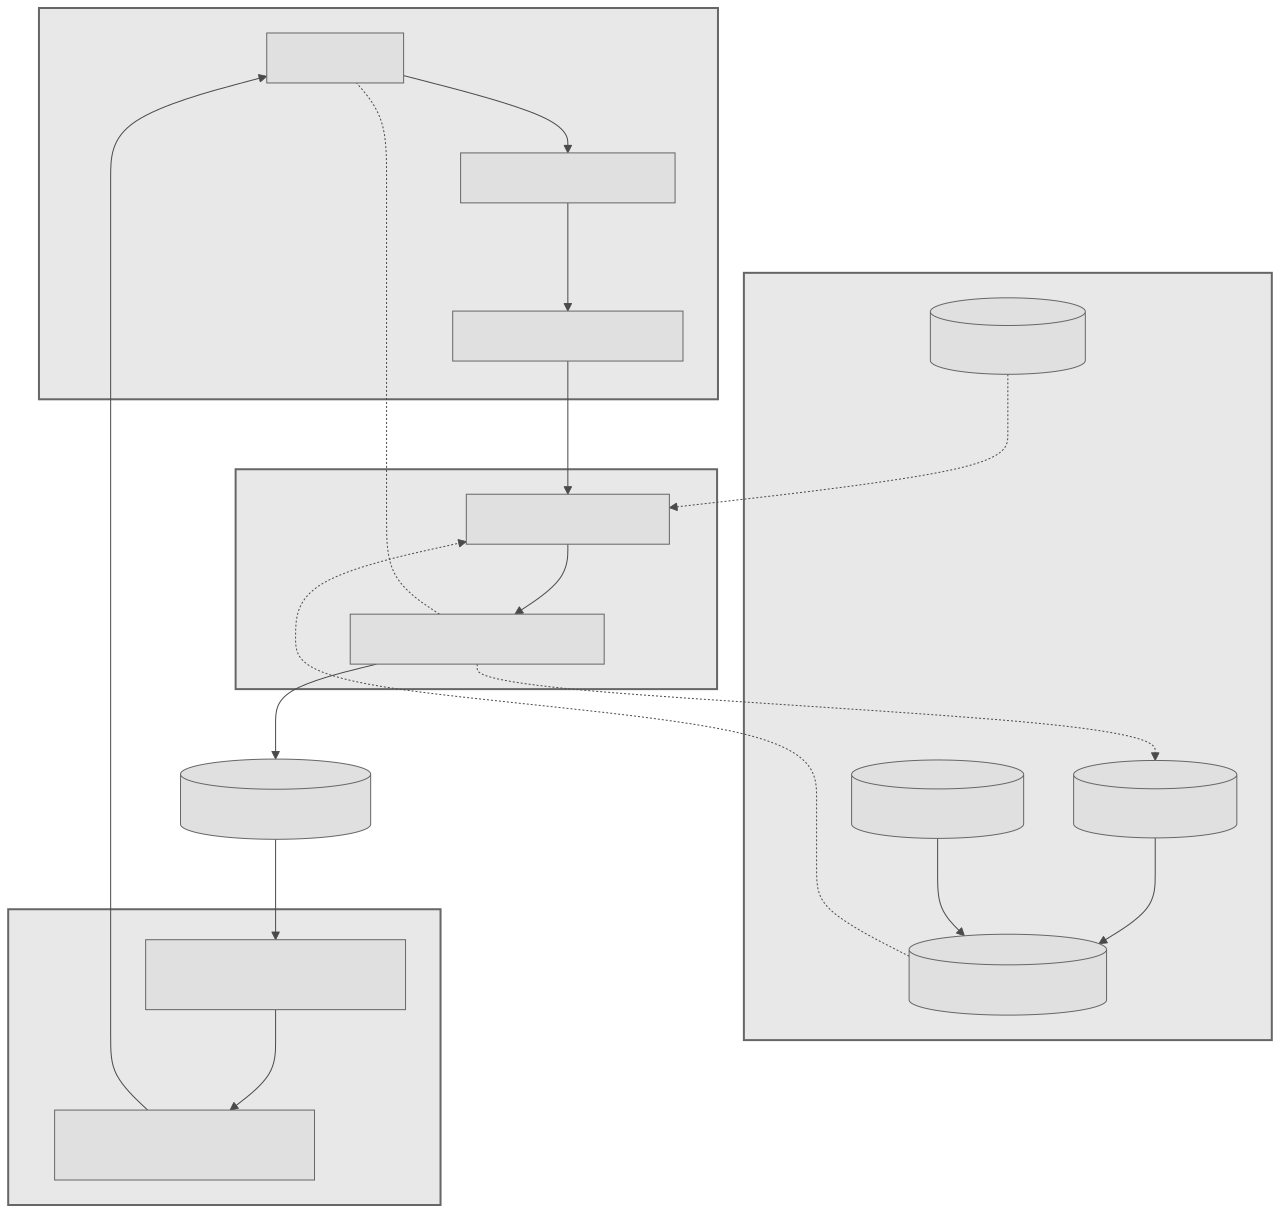
\includegraphics[width=0.95\textwidth,keepaspectratio]{figures/architecture.mmd.png}
\caption{Healthcare Analytics Architecture. Solid lines indicate the primary data flow from clinical user natural language queries through a conversational AI interface to a healthcare NLP engine for context-aware SQL generation against a healthcare data warehouse, ultimately delivering contextual insights with a feedback loop to the user. Dashed lines show knowledge injection paths where organizational memory and healthcare ontologies provide context and semantics to the NLP engine.}
\label{fig:architecture}
\end{figure}

\begin{enumerate}
\def\labelenumi{\arabic{enumi}.}
\setcounter{enumi}{2}
\tightlist
\item
  \textbf{Convergence Thesis}: We demonstrate that the simultaneous
  occurrence of technical advances in NL2SQL, low analytics maturity,
  and high workforce turnover creates conditions warranting
  organizational assessment. This convergence positions conversational
  AI as a potential mechanism for institutional knowledge preservation,
  though implementation decisions require organization-specific
  evaluation.
\end{enumerate}

\subsection{Document Structure}\label{document-structure}

Following this introduction, the paper proceeds through four main
sections. The Methodology section describes the narrative review
approach, literature search strategy, and source selection criteria. The
Literature Review synthesizes evidence across the three challenge
domains, establishing the current state of natural language processing
in healthcare, analytics maturity research, and workforce turnover
impacts. The Discussion examines implications, limitations, and future
research directions. Finally, the Conclusion summarizes the three-pillar
analytical framework as this paper's primary contribution to healthcare
informatics literature.

\section{Methodology}\label{methodology}

\subsection{Review Approach}\label{review-approach}

This paper employs a narrative review methodology to synthesize evidence
across three interconnected domains: healthcare analytics maturity,
workforce turnover, and natural language to SQL technologies. Unlike
systematic reviews that follow pre-registered protocols with exhaustive
searches, narrative reviews provide expert synthesis of relevant
literature to construct coherent arguments and identify patterns across
diverse evidence sources.

The narrative review approach was selected because:

\begin{enumerate}
\def\labelenumi{\arabic{enumi}.}
\tightlist
\item
  \textbf{Integration across domains}: The paper synthesizes evidence
  from distinct fields (clinical informatics, human resources, natural
  language processing) that require interpretive integration rather than
  statistical pooling
\item
  \textbf{Original analytical framework}: The three-pillar framework
  emerged iteratively from the literature rather than being
  pre-specified
\item
  \textbf{Heterogeneous evidence types}: The evidence base includes
  peer-reviewed research, industry reports, and benchmark datasets that
  cannot be meaningfully combined through meta-analysis
\end{enumerate}

\subsection{Literature Search}\label{literature-search}

Literature was identified through multiple channels between January 2023
and December 2025:

\textbf{Academic Databases:}

\begin{itemize}
\tightlist
\item
  Crossref: Cross-disciplinary academic literature, citation metadata
\item
  PubMed: Clinical informatics, healthcare workforce, medical
  administration
\item
  arXiv: Machine learning and NLP preprints, benchmark studies
\item
  Semantic Scholar: AI and computer science papers, citation analysis
\end{itemize}

\textbf{Industry Sources:}

\begin{itemize}
\tightlist
\item
  HIMSS: Analytics Maturity Model documentation and industry standards
\item
  Healthcare providers: NHS Trust implementation case studies
\item
  Market research: Precedence Research, Forrester analyst reports
\item
  Technology vendors: Health Catalyst, Oracle, Anthropic technical
  documentation
\item
  Professional associations: AHIMA/NORC workforce surveys
\item
  Business news: IBM, CNBC coverage of healthcare analytics ventures
\end{itemize}

\textbf{Search Concepts:}

Search terms were organized around the three-pillar framework:

\begin{itemize}
\tightlist
\item
  Analytics maturity: ``healthcare analytics maturity,'' ``HIMSS AMAM,''
  ``analytics adoption,'' ``analytics standardization failure,''
  ``low-code healthcare ROI,'' ``conversational AI platforms''
\item
  Workforce turnover: ``healthcare IT tenure,'' ``IT training time,''
  ``turnover cost salary,'' ``institutional memory loss,'' ``knowledge
  portal,'' ``knowledge capture,'' ``SECI model analytics''
\item
  Technical barriers: ``NL2SQL healthcare,'' ``text-to-SQL clinical,''
  ``MIMICSQL,'' ``EHRSQL,'' ``NL2SQL accuracy,'' ``NL2SQL
  productivity,'' ``schema discovery,'' ``PK/FK discovery,'' ``semantic
  column matching,'' ``vector embeddings schema''
\end{itemize}

\textbf{Search Results:}

Searches across all databases yielded 570 initial results after
deduplication. Crossref searches for terms including ``healthcare
analytics maturity,'' ``HIMSS AMAM,'' ``NL2SQL clinical,'' ``knowledge
portal,'' and ``low-code ROI'' (2015-current) returned 285 results, of
which 15 passed screening. PubMed searches combining workforce terms
(``healthcare IT tenure,'' ``IT training time,'' ``turnover cost
salary'') with analytics terms (``institutional memory,'' ``analytics
adoption,'' ``knowledge capture'') (2015-current) yielded 142 results
with 12 passing screening. arXiv searches in cs.CL and cs.DB categories
for ``text-to-SQL'' combined with technical terms (``MIMICSQL,''
``EHRSQL,'' ``schema discovery,'' ``PK/FK discovery,'' ``semantic
matching,'' ``vector embeddings'') (2020-current) produced 71 results
with 6 passing screening. Semantic Scholar searches for ``NL2SQL
healthcare,'' ``NL2SQL productivity,'' ``conversational AI clinical,''
and ``SECI model analytics'' (2015-current) returned 72 results with 8
passing screening. The final corpus includes 68 academic and 11 industry
sources (79 total).

Figure 2 illustrates the literature selection process, showing
progression from initial database search through screening and quality
assessment to the final corpus of 79 sources.

\begin{figure}[htbp]
\centering
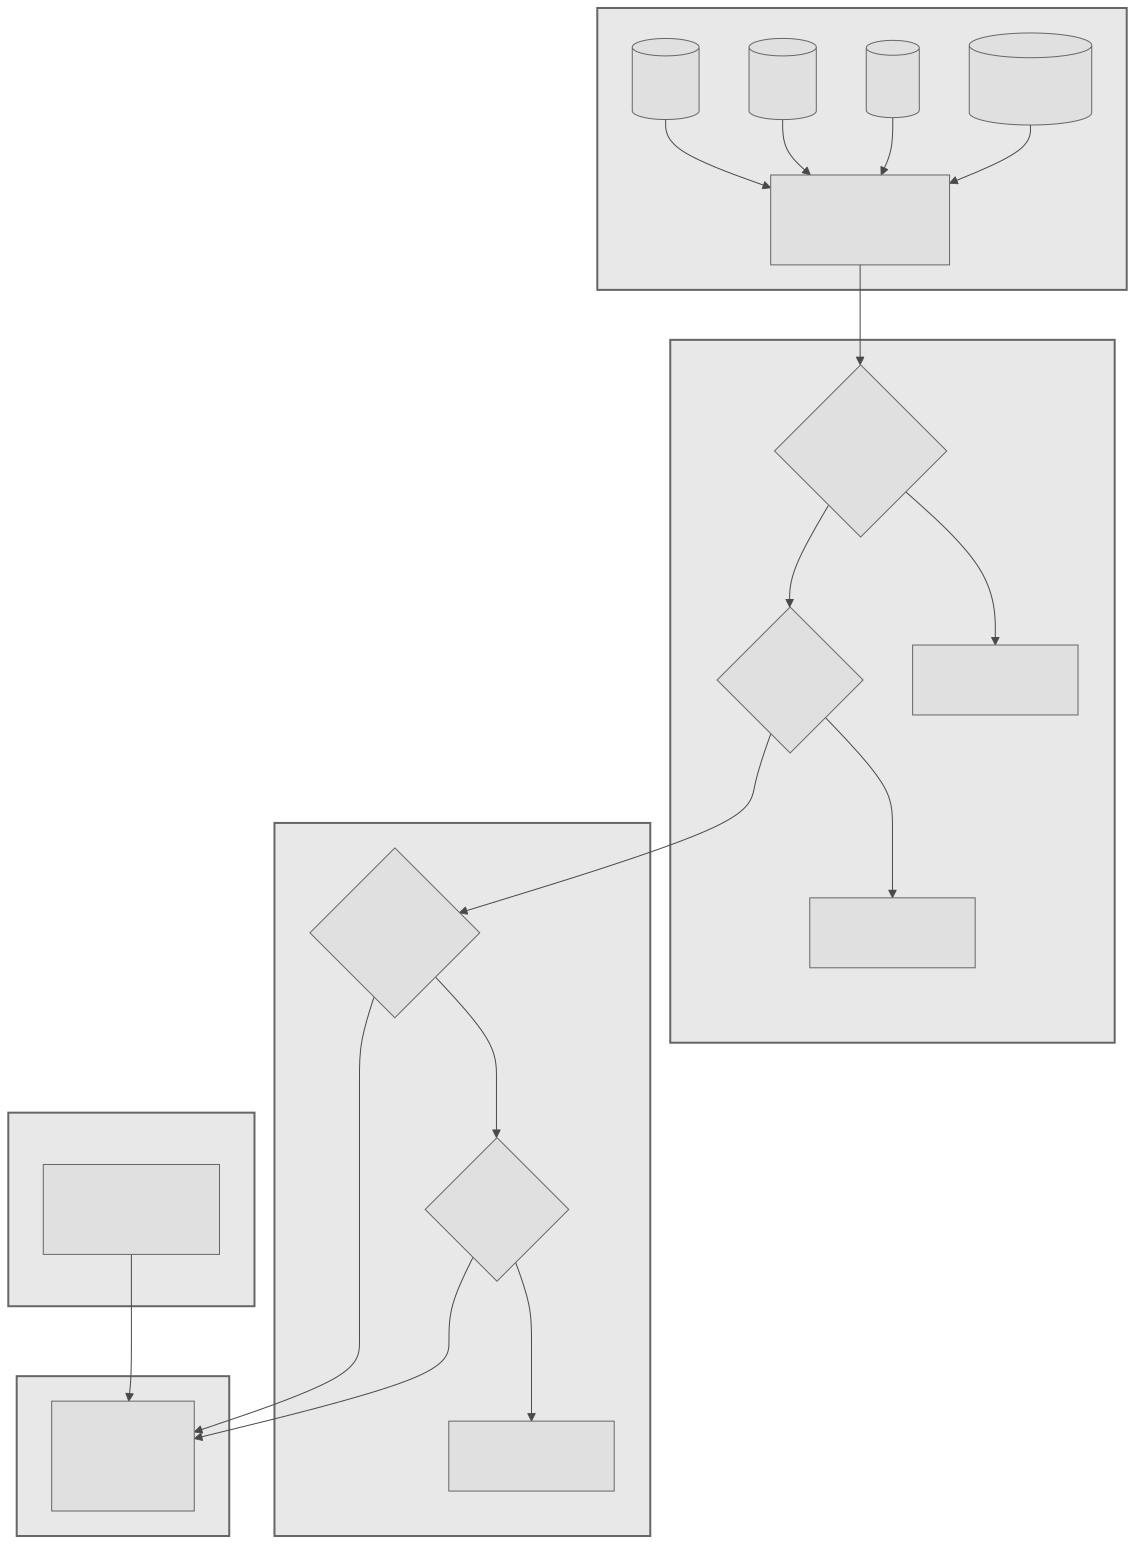
\includegraphics[width=0.9\textwidth,keepaspectratio]{figures/literature-flow.mmd.png}
\caption{Literature Selection Flow Diagram. The diagram shows the progression from initial database search (n ≈ 570) through title/abstract screening, full-text review, and quality assessment (AACODS for grey literature) to the final corpus of 79 sources (68 academic, 11 industry). Diagram source available in figures/literature-flow.mmd.}
\label{fig:literature-flow}
\end{figure}

\subsection{Source Selection}\label{source-selection}

Sources were selected based on the following criteria:

\textbf{Inclusion Criteria:}

\begin{itemize}
\tightlist
\item
  Peer-reviewed publications in healthcare informatics, medical
  informatics, computer science, or health services research
\item
  Industry reports from established healthcare IT organizations (HIMSS,
  AHIMA, AMIA)
\item
  Publications from 2015-current, with emphasis on 2020-current for
  rapidly evolving NL2SQL technologies
\item
  English language publications
\item
  Sources with verifiable DOIs, URLs, or institutional attribution
\end{itemize}

\textbf{Exclusion Criteria:}

\begin{itemize}
\tightlist
\item
  Sources without verifiable attribution or institutional backing
\item
  Vendor marketing materials without independent validation
\item
  Preprints without subsequent peer-reviewed publication (exception:
  foundational NL2SQL benchmarks where peer review is pending)
\item
  Studies with unverifiable statistics or methodological concerns
\end{itemize}

\subsection{Evidence Synthesis}\label{evidence-synthesis}

Evidence was synthesized thematically around the three-pillar framework:

\begin{enumerate}
\def\labelenumi{\arabic{enumi}.}
\tightlist
\item
  \textbf{Analytics maturity}: Evidence on HIMSS AMAM adoption,
  healthcare analytics capabilities, and organizational readiness
\item
  \textbf{Workforce turnover}: Evidence on nursing and IT staff turnover
  rates, institutional memory loss, and knowledge transfer challenges
\item
  \textbf{Technical barriers}: Evidence on NL2SQL benchmarks,
  healthcare-specific NLP challenges, and low-code implementation
  patterns
\end{enumerate}

This framework emerged iteratively from the literature rather than being
pre-specified, consistent with narrative review methodology.

\subsection{Grey Literature Quality
Assessment}\label{grey-literature-quality-assessment}

Grey literature sources were assessed using the AACODS checklist
{[}A30{]}, which evaluates Authority, Accuracy, Coverage, Objectivity,
Date, and Significance. Sources with vendor sponsorship were retained
when no independent alternative existed but flagged in-text. Table
\ref{tab:aacods} summarizes the assessment.

\begin{sidewaystable}
\centering
\caption{AACODS Assessment of Industry Sources}
\small
\begin{tabular}{|l|l|l|l|l|l|l|l|}
\hline
\textbf{Source} & \textbf{Authority} & \textbf{Accuracy} & \textbf{Coverage} & \textbf{Objectivity} & \textbf{Date} & \textbf{Significance} & \textbf{Include} \\
\hline
{[}I1{]} HIMSS AMAM & High$^\dagger$ & Verifiable & Global & High & 2024 & High & Yes \\
{[}I2{]} Snowdon/HIMSS & High$^\ddagger$ & Verifiable & N/A & High & 2024 & Medium & Yes \\
{[}I3{]} Health Catalyst & Medium$^\S$ & Unverifiable & US & Low & 2020 & Medium & Yes* \\
{[}I4{]} Berkshire NHS & High$^\P$ & Verifiable & Single site & High & 2024 & High & Yes \\
{[}I5{]} Forrester/Microsoft & Medium$^\|$ & Unverifiable & Enterprise & Low$^\diamondsuit$ & 2024 & Medium & Yes* \\
{[}I6{]} Oracle & Low$^\S$ & Unverifiable & N/A & Low & 2024 & Low & Yes* \\
{[}I7{]} Precedence Research & Medium$^\#$ & Unverifiable & Global & Medium & 2024 & Medium & Yes \\
{[}I8{]} Anthropic & Medium$^\S$ & Verifiable & N/A & Medium & 2025 & Low & Yes \\
{[}I9{]} IBM Newsroom & High$^{**}$ & Verifiable & N/A & High & 2022 & High & Yes \\
{[}I10{]} CNBC/Haven & High$^{**}$ & Verifiable & N/A & High & 2021 & High & Yes \\
{[}I11{]} AHIMA/NORC & High$^{\dagger\dagger}$ & Verifiable & US & High & 2023 & High & Yes \\
\hline
\end{tabular}
\label{tab:aacods}

\footnotesize
$^\dagger$Industry standards body.
$^\ddagger$HIMSS officer.
$^\S$Vendor.
$^\P$NHS trust.
$^\|$Analyst firm.
$^\#$Market research.
$^{**}$Journalism.
\\
$^{\dagger\dagger}$Professional association + academic.
$^\diamondsuit$Sponsor.
*Vendor sponsorship or low objectivity noted in manuscript text.
\end{sidewaystable}

\subsection{Methodological
Limitations}\label{methodological-limitations}

This narrative review has inherent limitations:

\begin{itemize}
\tightlist
\item
  \textbf{Non-exhaustive search}: Literature identification was
  selective rather than exhaustive; relevant studies may have been
  missed
\item
  \textbf{Limited formal quality assessment}: Grey literature sources
  were assessed using the AACODS checklist; however, no standardized
  quality assessment tool (e.g., GRADE, Cochrane Risk of Bias) was
  applied to peer-reviewed sources, as these tools are designed for
  clinical intervention studies rather than narrative reviews
\item
  \textbf{Single-coder bias risk}: Literature screening, data
  extraction, and thematic analysis were performed by a single author
  without independent verification. This introduces potential selection
  and interpretation bias that would be mitigated in systematic reviews
  through dual-coder protocols with inter-rater reliability assessment
\item
  \textbf{Post-hoc selection criteria}: Inclusion and exclusion criteria
  were refined during the review process rather than pre-registered
\item
  \textbf{No protocol registration}: This review was not registered in
  PROSPERO or similar registries
\item
  \textbf{Dated workforce statistics}: The primary healthcare IT
  turnover statistic (34\% annually) derives from Ang and Slaughter's
  2004 study {[}A10{]}. While recent surveys confirm workforce
  challenges persist {[}I11{]} and contemporary evidence suggests the
  situation may have worsened (55\% intent to leave among public health
  informatics specialists {[}A66{]}), no study has directly replicated
  the 2004 tenure measurement methodology. Future research should
  address this methodological gap
\end{itemize}

These limitations are balanced against the strengths of narrative review
methodology: ability to synthesize heterogeneous evidence types across
disciplinary boundaries, flexibility to pursue emerging themes, and
capacity to construct novel analytical frameworks that illuminate
connections between previously disconnected research domains.

\section{Framework Development and
Validation}\label{framework-development-and-validation}

This paper's primary contribution is the three-pillar analytical
framework for understanding healthcare analytics challenges: (1)
analytics maturity gaps, (2) workforce turnover and institutional memory
loss, and (3) technical barriers in natural language to SQL generation.
This section documents the framework's development process and
theoretical grounding.

\subsection{Framework Development
Process}\label{framework-development-process}

The three-pillar framework emerged through iterative analysis of the
literature corpus. Initial review identified numerous disconnected
research streams: NL2SQL technical advances, HIMSS maturity models,
healthcare workforce turnover studies, knowledge management theory, and
healthcare IT implementation case studies. These appeared as isolated
topics until thematic analysis revealed recurring patterns of
interdependence.

The framework development followed these steps:

\begin{enumerate}
\def\labelenumi{\arabic{enumi}.}
\tightlist
\item
  \textbf{Theme Extraction}: Systematic coding of 79 sources identified
  recurring themes across technical, organizational, and workforce
  dimensions
\item
  \textbf{Pattern Recognition}: Cross-domain analysis revealed that
  challenges in each dimension amplified challenges in others (e.g.,
  workforce turnover degrading analytics maturity, technical barriers
  preventing knowledge capture)
\item
  \textbf{Pillar Identification}: Three orthogonal yet interconnected
  dimensions emerged as the organizing structure:

  \begin{itemize}
  \tightlist
  \item
    \textbf{Analytics Maturity}: Organizational capability progression
    measured against HIMSS AMAM stages
  \item
    \textbf{Workforce Dynamics}: Human capital retention and tacit
    knowledge preservation
  \item
    \textbf{Technical Barriers}: NL2SQL capabilities and
    healthcare-specific implementation challenges
  \end{itemize}
\item
  \textbf{Framework Validation}: Pillar structure tested against all 79
  sources to confirm comprehensive coverage without significant gaps
\end{enumerate}

\subsection{Theoretical Grounding}\label{theoretical-grounding}

The three-pillar framework aligns with established models in healthcare
informatics and knowledge management:

\begin{table}[htbp]
\centering
\caption{Framework Alignment with Established Models}
\label{tab:framework-alignment}
\begin{tabular}{p{3cm}p{3.5cm}p{3.5cm}p{3.5cm}}
\toprule
\textbf{Three Pillars} & \textbf{HIMSS AMAM Alignment} & \textbf{DIKW Hierarchy} & \textbf{Knowledge Management} \\
\midrule
Analytics Maturity & Stages 0-7 progression & Data \newline → Information & Organizational learning \\
Workforce Dynamics & Implicit in advanced stages & Knowledge (tacit) \newline → Wisdom & Tacit knowledge transfer \\
Technical Barriers & Stage 6-7 requirements & Information \newline → Knowledge & Knowledge codification \\
\bottomrule
\end{tabular}
\end{table}

The HIMSS Analytics Maturity Assessment Model {[}I1{]} provides
organizational benchmarks but does not explicitly address workforce
knowledge retention. The Data-Information-Knowledge-Wisdom (DIKW)
hierarchy explains the progression from raw data to actionable insight,
but standard formulations do not address institutional memory loss. The
three-pillar framework synthesizes these perspectives, positioning
workforce dynamics as the critical enabler connecting data access
(analytics maturity) with organizational wisdom (knowledge
preservation).

\subsection{Framework Scope and
Limitations}\label{framework-scope-and-limitations}

The framework is descriptive rather than prescriptive; it provides an
analytical lens for understanding healthcare analytics challenges but
does not mandate specific solutions. Future research should empirically
validate pillar interdependencies through longitudinal organizational
studies and develop quantitative metrics for framework dimensions.

\section{Literature Review: Natural Language Analytics in Healthcare -
Evidence for Institutional Memory
Preservation}\label{literature-review-natural-language-analytics-in-healthcare---evidence-for-institutional-memory-preservation}

This narrative review examines evidence supporting the implementation of
natural language analytics platforms in healthcare systems. Drawing from
peer-reviewed research, industry reports, and benchmark datasets
identified through the methodology described in Section 2 (Methodology),
we synthesize findings across three domains. Analysis reveals three
critical findings: (1) natural language to SQL generation has evolved
significantly but faces healthcare-specific challenges requiring
specialized solutions, (2) healthcare analytics maturity remains low
with most organizations struggling at basic stages, and (3) healthcare
workforce turnover creates institutional memory loss that traditional
approaches fail to address. The evidence strongly supports
conversational AI platforms as a solution to these interconnected
challenges.

\subsection{Current State of Natural Language to SQL
Generation}\label{current-state-of-natural-language-to-sql-generation}

\subsubsection{Evolution and Technical
Advances}\label{evolution-and-technical-advances}

Recent systematic reviews document the rapid evolution of natural
language to SQL (NL2SQL) technologies. Ziletti and D'Ambrosi {[}A6{]}
demonstrate that retrieval augmented generation (RAG) approaches
significantly improve query accuracy when applied to electronic health
records (EHRs), though they note that ``current language models are not
yet sufficiently accurate for unsupervised use'' in clinical settings.
Their work on the MIMIC-3 dataset shows that integrating medical coding
steps into the text-to-SQL process improves performance over simple
prompting approaches.

Recent benchmarking studies {[}A8{]}, {[}A9{]} examining LLM-based
systems for healthcare identify unique challenges: medical terminology,
characterized by abbreviations, synonyms, and context-dependent
meanings, remains a barrier to accurate query generation. Evaluations of
state-of-the-art LLMs including GPT-4 and Claude 3.5 show that even
top-performing models achieve only 69-73\% accuracy on clinical tasks,
with significant gaps remaining between benchmark performance and real
clinical readiness.

\subsubsection{Healthcare-Specific
Challenges}\label{healthcare-specific-challenges}

The literature consistently identifies domain-specific obstacles in
healthcare NL2SQL implementation. A systematic review of NLP in EHRs
{[}A4{]} found that the lack of annotated data, automated tools, and
other challenges hinder the full utilization of NLP for EHRs. The
review, following PRISMA guidelines, categorized healthcare NLP
applications into seven areas, with information extraction and clinical
entity recognition proving most challenging due to medical terminology
complexity.

Wang et al.~{[}A5{]} demonstrate that healthcare NL2SQL methods must
move beyond the constraints of exact or string-based matching to fully
encompass the semantic complexities of clinical terminology. This work
emphasizes that general-purpose language models fail to capture the
nuanced relationships between medical concepts, diagnoses codes (ICD),
procedure codes (CPT), and medication vocabularies (RxNorm).

\subsubsection{Promising Approaches and
Limitations}\label{promising-approaches-and-limitations}

Recent advances show promise in addressing these challenges. The
TREQS/MIMICSQL dataset development {[}A5{]} and EHRSQL benchmark
{[}A3{]} provide question-SQL pairs specifically for healthcare,
featuring questions in natural, free-form language. This approach
acknowledges that healthcare queries often require multiple logical
steps: population selection, temporal relationships, aggregation
statistics, and mathematical operations.

However, significant limitations persist. Benchmarking studies {[}A8{]},
{[}A9{]} conclude that while LLMs show capability in healthcare tasks,
most models struggle with complex clinical reasoning. The MedAgentBench
evaluation found even the best-performing model (Claude 3.5 Sonnet)
achieved only 69.67\% success rate on medical agent tasks, highlighting
the gap between current capabilities and clinical readiness.

\subsubsection{Productivity and Efficiency
Evidence}\label{productivity-and-efficiency-evidence}

Emerging research documents quantifiable productivity gains from NL2SQL
implementations. In healthcare settings, organizations implementing
natural language interfaces report a 63\% increase in self-service
analytics adoption among non-technical staff and a 37\% reduction in
time spent on data retrieval tasks {[}A36{]}. Business analysts using
these interfaces spend 42\% more time on analysis rather than query
construction {[}A36{]}.

Clinical-specific natural language interfaces demonstrate significant
efficiency improvements. Criteria2Query, a natural language interface
for clinical database cohort definition, achieves fully automated query
formulation in an average of 1.22 seconds per criterion, enabling
researchers to query EHR data without mastering database query languages
{[}A35{]}. User studies show NL2SQL systems reduce query completion
times by 10-30\% compared to traditional SQL platforms while improving
accuracy from 50\% to 75\%, with users recovering from errors 30-40
seconds faster {[}A38{]}.

The most substantial productivity gains appear in multimodal interfaces.
Research on speech-driven database querying demonstrates users can
specify SQL queries with an average speedup of 2.7x (up to 6.7x)
compared to traditional input methods, with user effort reduced by a
factor of 10x to 60x compared to raw typing {[}A37{]}.
Healthcare-specific natural language query systems show dramatic
improvements: a clinical data analytics language (CliniDAL) reduced
complex query formulation from ``many days'' with SQL to ``a few hours''
with natural language, with expert users describing SQL as ``very
tedious and time-consuming'' for the same analytical tasks {[}A43{]}.
NLP-driven data entry systems have achieved 33\% time reduction with
15\% accuracy improvement in clinical research settings {[}A44{]}.
Healthcare-specific NL2SQL models such as MedT5SQL achieve 80.63\% exact
match accuracy on the MIMICSQL benchmark, demonstrating that
domain-adapted language models can effectively translate natural
language to SQL for clinical databases {[}A45{]}. These metrics provide
peer-reviewed evidence that complements vendor-sponsored efficiency
claims.

Code modernization principles directly inform these productivity gains.
Foundational work on natural language interfaces to databases {[}A46{]}
established that modular, decoupled architecture enables effective NL
access to legacy systems, a design principle validated across 47 years
of subsequent research. Modern implementations demonstrate that
retrieval-augmented generation (RAG) approaches reduce specialized
training requirements by 87.4\% compared to traditional querying methods
while achieving 92.3\% accuracy in interpreting business-specific
terminology from legacy mainframe records {[}A49{]}. This convergence of
code modernization and natural language interface technologies arises
because both rely on the same underlying large language models
{[}A47{]}, {[}A48{]}, suggesting that organizations investing in either
capability simultaneously advance both.

\subsection{State of Healthcare Analytics
Maturity}\label{state-of-healthcare-analytics-maturity}

\subsubsection{Low Organizational
Maturity}\label{low-organizational-maturity}

The Healthcare Information Management Systems Society (HIMSS) Analytics
Maturity Assessment Model (AMAM) provides the industry standard for
measuring analytics capabilities. Recent data reveals a concerning state
of analytics maturity in healthcare organizations globally {[}I1{]}. The
newly revised AMAM24 model, launched in October 2024, represents a
significant evolution from the original framework.

Snowdon {[}I2{]}, Chief Scientific Research Officer at HIMSS, emphasizes
that ``analytics as a discipline has changed dramatically in the last
five to 10 years,'' yet healthcare organizations struggle to keep pace
{[}A14{]}. Research confirms healthcare's adoption of analytics often
lags behind other sectors such as retail and banking, partly due to the
complexity of implementing new technology in clinical environments. The
newly revised AMAM model shifts focus from technical capabilities to
outcomes, measuring the real impact of analytics on patient care,
system-wide operations, and governance.

Quantitative evidence links analytics maturity directly to patient
outcomes. Cross-sectional studies using the HIMSS Electronic Medical
Record Adoption Model (EMRAM) demonstrate that hospitals with advanced
digital maturity (levels 6-7) have 3.25 times higher odds of achieving
better Leapfrog Group Hospital Safety Grades compared to hospitals at
EMRAM level 0, with significantly reduced infection rates and fewer
adverse events {[}A54{]}. Similarly, high-maturity hospitals have 1.8 to
2.24 times higher odds of achieving higher patient experience ratings
{[}A55{]}. Big data analytics capabilities, combined with complementary
organizational resources and analytical personnel skills, improve
readmission rates and patient satisfaction {[}A56{]}, while poor-quality
data (a component of lower maturity) results in diagnostic errors,
ineffective treatments, and compromised patient care {[}A57{]}.

\subsubsection{Barriers to Analytics
Adoption}\label{barriers-to-analytics-adoption}

A systematic literature review of big data analytics in healthcare by
Kamble et al.~{[}A7{]} identifies critical barriers to analytics
adoption. The study reveals that healthcare enterprises struggle with
technology selection, resource allocation, and organizational readiness
for data-driven decision making.

Health Catalyst's Healthcare Analytics Adoption Model {[}I3{]}, a
vendor-produced framework, corroborates these findings, documenting that
most healthcare organizations remain at Stages 0-3, characterized by:

\begin{itemize}
\tightlist
\item
  Fragmented data sources without integration
\item
  Limited automated reporting capabilities
\item
  Lack of standardized data governance
\item
  Minimal predictive or prescriptive analytics
\item
  Absence of real-time decision support
\end{itemize}

\subsubsection{The Analytics Skills Gap}\label{the-analytics-skills-gap}

The literature consistently identifies workforce capabilities as a
primary constraint. Healthcare organizations face mounting challenges in
extracting meaningful insights from the vast amount of unstructured
clinical text data generated daily {[}A4{]}. There is an acknowledged
problem in health services where organizations cannot make good use of
available data due to a deficit in skilled analysts across all sectors
and levels {[}A15{]}. Organizations face critical challenges in
recruiting and retaining professionals with the right analytical skills,
while the need for big data specialists with analytical capabilities
continues to grow {[}A16{]}. Traditional approaches to analytics require
extensive technical expertise and time that healthcare professionals
typically lack, creating a fundamental barrier to analytics adoption
{[}I11{]}.

\subsection{Healthcare Workforce Turnover and Knowledge
Loss}\label{healthcare-workforce-turnover-and-knowledge-loss}

\subsubsection{Turnover Rates and Financial
Impact}\label{turnover-rates-and-financial-impact}

Multiple meta-analyses provide comprehensive data on healthcare
workforce turnover. Wu et al.~{[}A1{]} found a pooled prevalence of
nurse turnover at 18\% (95\% CI: 11-26\%), with rates varying from
11.7\% to 46.7\% across different countries and settings. Ren et
al.~{[}A2{]} corroborated these findings with a global nurse turnover
rate ranging from 8\% to 36.6\%, with a pooled rate of 16\% (95\% CI:
14-17\%).

The financial implications are substantial. Massingham {[}A24{]}
measured the impact of knowledge loss in a longitudinal study, finding
that the total financial cost to address problems caused by knowledge
loss reached three times the organization's annual salary budget,
including increased training costs, productivity losses, and project
delays. Healthcare-specific evidence quantifies replacement costs in
absolute terms: replacing a primary care clinician costs healthcare
organizations over \$500,000 due to lost revenue and recruiting expenses
{[}A67{]}, while physician replacement can reach up to \$1 million per
departure, with national annual costs estimated at \$4.6 billion
{[}A68{]}. Vendor analysis from Oracle {[}I6{]} corroborates these
findings, documenting turnover costs at 0.5-2.0 times annual salary with
knowledge-intensive positions reaching the higher end.

Technical and analytics staff face even more severe turnover challenges.
In their 2004 study, Ang and Slaughter {[}A10{]} found that IT
professionals at healthcare provider institutions (where IT serves as a
support function rather than core business) had average tenure of just
2.9 years, implying annual turnover of 34\% (calculated as 1/2.9 years),
the highest rate among all IT organization types studied at that time.
This compared unfavorably to the 9.68-year average for IT managerial
positions overall. While this data is now two decades old, contemporary
evidence suggests the turnover challenge persists or has worsened. A
2025 analysis of nationally representative US survey data (n=44,732)
found that 55\% of public health informatics specialists intended to
leave their positions {[}A66{]}. The 2023 AHIMA/NORC workforce survey
found that 66\% of health information professionals report persistent
staffing shortages, with 83\% witnessing increased unfilled positions
over the past year {[}I11{]}.

The knowledge loss implications are substantial. Research documents
significant time-to-productivity requirements across healthcare IT
roles: basic EHR training requires 8 hours to 2 months for end-users,
while health information workforce development demands 18 months to 2
years for specialized roles {[}A11{]}. International Medical Informatics
Association recommendations specify a minimum of 1 year (60 ECTS
credits) for biomedical and health informatics specialists {[}A12{]},
with personalized EHR training programs requiring 6 months of blended
instruction to achieve meaningful competency improvements {[}A13{]}.
Combined with the 2.9-year average tenure, healthcare IT professionals
may operate at full productivity for only approximately two years before
departing. This creates a perpetual cycle where organizations lose
experienced staff before fully recouping their training investment.

The impact on care continuity is well-documented. Clinical handover
disruption is internationally recognized as a patient safety priority
because it represents a fundamental disruption to continuity of care and
is prone to errors {[}A58{]}. Empirical studies demonstrate that nursing
unit turnover reduces workgroup learning and is associated with
increased patient falls, medication errors, and reduced patient
satisfaction {[}A59{]}. International evidence links high workforce
turnover to poorer continuity of care, particularly in remote health
services, with measurable outcomes including increased hospitalizations
and years of life lost {[}A60{]}. When senior executives and knowledge
workers depart, organizations experience ``corporate memory loss'' that
undermines organizational continuity and effectiveness {[}A61{]}.

\subsubsection{Institutional Memory
Loss}\label{institutional-memory-loss}

The concept of institutional memory in healthcare has received
increasing attention. Institutional memory encompasses the collective
knowledge, experiences, and expertise that enables organizational
effectiveness. Healthcare organizations typically lack formal mechanisms
for knowledge preservation, relying instead on person-to-person transfer
that fails during rapid turnover. Cultural and regulatory obstacles for
data sharing further limit the ability of healthcare organizations to
achieve the full potential of their data assets {[}A17{]}.

When experienced analysts, clinical informatics professionals, or
data-savvy clinicians leave, they take with them irreplaceable knowledge
about data definitions, business rules, analytical approaches, and
organizational context. Research on tacit knowledge transfer provides
strong evidence that this knowledge is inherently difficult to document
through traditional means. Empirical studies demonstrate that learning
related to tacit knowledge is often not captured in formal post-project
review reports {[}A50{]}, and conventional mechanisms such as documents,
blueprints, and procedures fail because tacit knowledge is not easily
codified {[}A51{]}. Research across multiple industries consistently
shows that written reports and databases fail to convey key learning
from expert teams {[}A52{]}, while experts often lack the skills,
motivation, or time to document their expertise, and even when
documentation is attempted, essential aspects are lost due to lack of
shared experience between experts and novices {[}A53{]}.

\subsubsection{Inadequacy of Traditional
Approaches}\label{inadequacy-of-traditional-approaches}

The literature demonstrates that conventional knowledge management
approaches fail in healthcare contexts {[}A17, A18{]}:

\begin{itemize}
\tightlist
\item
  Traditional knowledge transfer mechanisms show limited effectiveness
\item
  Organizations struggle to capture and maintain analytical expertise
\item
  Security concerns and employee resistance to change slow the pace of
  information system acceptance {[}A18{]}
\item
  Person-to-person knowledge transfer fails during rapid turnover cycles
\end{itemize}

\subsection{Integration of Evidence: The Case for Conversational
AI}\label{integration-of-evidence-the-case-for-conversational-ai}

\subsubsection{Bridging Technical and Domain
Expertise}\label{bridging-technical-and-domain-expertise}

At its core, bridging technical and domain expertise serves a
fundamental patient care objective: enabling clinical professionals to
access and act on data that improves care quality. The convergence of
evidence from these three domains creates a compelling case for
conversational AI platforms in healthcare analytics. Natural language
interfaces directly address the technical barriers identified in the
literature by eliminating the need for SQL expertise while preserving
the sophisticated query capabilities required for healthcare data.

Low-code platforms and conversational AI represent complementary
approaches to reducing technical barriers in healthcare analytics.
Low-code platforms provide visual development environments that
accelerate application development and reduce coding requirements, while
conversational AI enables natural language interaction with data
systems. These approaches share core benefits: both democratize access
by enabling non-technical users to perform complex analyses previously
requiring data scientist intervention, both accelerate development
cycles by abstracting technical complexity, and both produce more
self-documenting systems where business logic is expressed in accessible
formats rather than specialized code. Evidence from low-code
implementations thus informs conversational AI adoption, as both address
the same fundamental barrier: the gap between clinical expertise and
technical capability.

\subsubsection{Knowledge Preservation
Mechanisms}\label{knowledge-preservation-mechanisms}

The literature suggests that effective knowledge preservation requires
active, embedded systems rather than passive documentation. AI-based
platforms can serve as organizational memory systems by:

\begin{itemize}
\tightlist
\item
  Capturing decision-making patterns through usage
\item
  Encoding best practices in accessible formats
\item
  Providing context-aware guidance to new users
\item
  Maintaining knowledge currency through continuous learning
\end{itemize}

These principles align with conversational AI approaches that embed
institutional knowledge within the AI model itself, making expertise
permanently accessible regardless of staff turnover.

\subsubsection{Empirical Support for Barrier-Reducing
Technologies}\label{empirical-support-for-barrier-reducing-technologies}

Academic research provides growing evidence for both conversational AI
and low-code approaches in healthcare, technologies that share the goal
of reducing technical barriers to data-driven decision making. A
foundational systematic review of AI conversational agents in healthcare
{[}A39{]} established that such systems reduce burden on healthcare
resources and save providers' time, though the review identified a need
for more rigorous quantitative validation. Subsequent RCT-based
systematic reviews provide this evidence: a meta-analysis of
conversational agent interventions reported mean task completion rates
of 83\% (range 40-100\%) across healthcare applications {[}A41{]}.
Real-world validation at scale comes from a study of conversational AI
across nine NHS mental health services involving 64,862 patients,
demonstrating reduced clinician assessment time, shorter patient wait
times, and lower dropout rates {[}A42{]}. On the clinical AI side,
Sezgin et al.~{[}A19{]} demonstrated that GPT-3-powered chatbots can
reduce overhead at clinics, while Jiao et al.~{[}A20{]} found AI
adoption leads to cost savings through improved service delivery and
shorter hospitalization lengths. Dai and Abramoff {[}A21{]} explain that
AI generates predictions affordably, enabling earlier care that
potentially prevents costly interventions.

Low-code implementations provide parallel evidence for the benefits of
barrier reduction. Berkshire Healthcare NHS Trust {[}I4{]} reports over
800 ``citizen developers'' (and over 1,600 total users) now creating
solutions using Microsoft Power Platform. The NHS program demonstrates
that healthcare professionals without IT expertise can use low-code
tools to create custom solutions and apps, streamlining operations and
enabling data-driven decisions. This evidence supports the broader
principle that reducing technical barriers, whether through visual
development or natural language interfaces, enables healthcare domain
experts to leverage data directly. A systematic literature review of 17
peer-reviewed papers identified cost and time minimization as the most
frequently discussed benefits of low-code development, with healthcare
among the primary implementation domains {[}A31{]}. Controlled
experiments quantify these benefits: a comparative study of traditional
versus low-code development for a healthcare cognitive rehabilitation
system found low-code required 47.5 hours versus 888 hours for
traditional development, representing a 94.63\% reduction in effort
{[}A40{]}. Industry-sponsored research from Forrester {[}I5{]} projects
206\% three-year ROI from low-code implementations; peer-reviewed
studies report similar findings, with healthcare institutions achieving
177\% ROI over 36 months while reducing development time by 67\% and
technical resource requirements by 58\% {[}A33{]}, and small healthcare
clinics achieving 250\% cumulative ROI over three years {[}A34{]}.

Healthcare-specific studies show concrete benefits across both
approaches: Pennington {[}A22{]} found AI in revenue cycle management
accelerated payment cycles from 90 days to 40 days, while Atobatele et
al.~{[}A23{]} documented how low-code platforms enable non-technical
staff to build applications, leading to efficiency gains. Rapid
application development using low-code characteristics enabled an
mHealth app for COVID-19 remote care that saved 2,822 hospital bed-days
for 400 enrolled patients {[}A32{]}. These findings collectively
demonstrate that technologies enabling non-technical users to interact
with complex systems, whether through visual interfaces or natural
language, produce measurable organizational benefits.

\subsection{Implications for Healthcare
Organizations}\label{implications-for-healthcare-organizations}

\subsubsection{Strategic Alignment with Industry
Trends}\label{strategic-alignment-with-industry-trends}

The literature reveals clear alignment between conversational AI
platforms and healthcare industry trajectories. The revised HIMSS AMAM
model {[}I1{]} explicitly emphasizes AI readiness and governance
frameworks that natural language platforms inherently support.
Organizations implementing such platforms can advance multiple maturity
stages simultaneously by democratizing analytics while maintaining
governance.

\subsubsection{Return on Investment
Evidence}\label{return-on-investment-evidence}

Academic research documents multiple pathways to ROI for
barrier-reducing technologies in healthcare. Conversational AI
implementations show direct benefits: Jiao et al.~{[}A20{]} found that
AI-driven efficiency gains, including shorter hospitalization lengths,
translate into financial and operational benefits for healthcare
providers; Pennington {[}A22{]} documented that AI in revenue cycle
management accelerated payment cycles from 90 to 40 days, improving cash
flow; and Sezgin et al.~{[}A19{]} proposed chatbot implementations that
reduce clinic overhead.

Low-code platform ROI provides analogous evidence for the value of
technical barrier reduction. Industry-sponsored research from Forrester
{[}I5{]} projects 206\% three-year ROI from Power Platform
implementations. Peer-reviewed studies corroborate these findings: a
systematic review identified cost and time reduction as the most
frequently discussed benefits across 17 studies {[}A31{]}, healthcare
institutions report 177\% ROI over 36 months with 67\% faster
development {[}A33{]}, and small healthcare clinics document 250\%
cumulative three-year ROI {[}A34{]}. While low-code and conversational
AI differ in implementation approach, both generate returns through the
same mechanism: enabling domain experts to accomplish tasks previously
requiring specialized technical staff. Market research supports
continued investment in accessible analytics: Precedence Research
{[}I7{]} projects the healthcare analytics market to grow from \$64.49
billion in 2025 to \$369.66 billion by 2034 (21.41\% CAGR).

\subsubsection{Risk Mitigation Through Knowledge
Preservation}\label{risk-mitigation-through-knowledge-preservation}

The literature emphasizes that institutional memory loss represents an
existential risk to healthcare analytics programs. Conversational AI
platforms mitigate this risk by transforming tacit knowledge into
encoded, accessible expertise. This approach aligns with best practices
for embedding organizational knowledge in systems rather than
individuals, ensuring continuity despite workforce turnover.

\subsection{Gaps in Current
Literature}\label{gaps-in-current-literature}

Despite substantial evidence supporting conversational AI in healthcare
analytics, several research gaps persist:

\begin{enumerate}
\def\labelenumi{\arabic{enumi}.}
\tightlist
\item
  \textbf{Long-term outcomes}: Most studies examine 6-24 month
  implementations; multi-year impacts remain understudied
\item
  \textbf{Scalability across specialties}: Evidence primarily focuses on
  general acute care; specialty-specific applications need investigation
\item
  \textbf{Governance frameworks}: Limited research on optimal governance
  models for democratized analytics
\item
  \textbf{Training methodologies}: Best practices for transitioning from
  traditional to conversational analytics lack empirical validation
\item
  \textbf{Integration patterns}: Architectural guidance for
  incorporating conversational AI into existing healthcare IT ecosystems
  remains sparse
\item
  \textbf{Long-term productivity tracking}: While peer-reviewed studies
  now document immediate productivity gains (63\% self-service adoption
  increase, 37\% data retrieval time reduction, 10-30\% query completion
  time improvement {[}A35{]}, {[}A36{]}, {[}A37{]}, {[}A38{]}),
  longitudinal studies tracking sustained productivity improvements over
  multiple years remain limited
\end{enumerate}

\subsection{Why the Problem Persists}\label{why-the-problem-persists}

Despite clear evidence of healthcare's analytics challenges and
available technology, the problem remains unsolved. Analysis of market
dynamics reveals three structural barriers:

\subsubsection{Failed Standardization
Approaches}\label{failed-standardization-approaches}

Large-scale efforts to standardize healthcare data and analytics have
consistently encountered fundamental barriers. Academic research
identifies a persistent tension between achieving short-term
institutional solutions and pursuing long-term global interoperability,
with standardization complexity arising from diverse community interests
and technical issues {[}A26{]}. Data standardization faces three primary
technological obstacles: metadata uncertainties, data transfer
challenges, and missing data, compounded by legacy data collection
methods that have created a ``patchwork'' of inconsistent organizational
practices {[}A27{]}.

These challenges manifest in clinical practice through workflow
variability. Even within the same institution, clinical workflows vary
significantly, and transitions to standardized systems often cause
profound disruptions to existing processes {[}A28{]}. At the
institutional level, data fragmentation across different organizations
creates barriers to linkage, access, and care continuity, while
governance issues including unclear responsibilities and weak
collaboration compound the problem {[}A29{]}.

High-profile industry events illustrate these documented challenges. IBM
divested its Watson Health data and analytics assets in 2022 {[}I9{]},
and the Haven healthcare venture (backed by Amazon, Berkshire Hathaway,
and JPMorgan Chase) disbanded in 2021 after three years {[}I10{]}. These
outcomes align with the academic literature's findings: standardized
solutions face significant barriers when applied across institutions
with unique data definitions, business rules, and clinical workflows.

These observations represent documented market events; however,
establishing causal mechanisms between organizational strategies and
interoperability outcomes requires controlled empirical research beyond
this review's scope. The patterns noted here warrant further
investigation through rigorous organizational studies.

\subsubsection{Deployment Constraint
Mismatch}\label{deployment-constraint-mismatch}

Healthcare organizations increasingly require solutions functional in
secure, air-gapped environments due to regulatory requirements and data
governance policies. General-purpose cloud AI services cannot meet these
deployment constraints while simultaneously lacking the
institution-specific context necessary for accurate analytics. The
fundamental requirement that institutional knowledge must be captured,
preserved, and accessed within each organization's specific environment
cannot be addressed by standardized cloud offerings.

These dynamics explain why, despite technological capability, the
healthcare analytics maturity gap persists. Solutions must be designed
for institution-specific deployment rather than cross-organizational
standardization.

\section{Discussion}\label{discussion}

\subsection{Strengths of the Evidence
Base}\label{strengths-of-the-evidence-base}

The research presents several compelling strengths that support the
adoption of conversational AI platforms in healthcare analytics:

\subsubsection{Validated Benchmarking
Data}\label{validated-benchmarking-data}

The evidence base includes peer-reviewed benchmarking studies from top
venues (NEJM AI, NeurIPS, NAACL) that provide empirical validation of
LLM capabilities in healthcare contexts. Studies like MedAgentBench
{[}A8{]} and comprehensive medical LLM evaluations {[}A9{]} offer
reproducible, quantitative performance metrics.

\subsubsection{Real-World Implementation
Evidence}\label{real-world-implementation-evidence}

The Berkshire Healthcare NHS Trust case {[}I4{]} demonstrates successful
low-code adoption in healthcare, with over 800 citizen developers
creating solutions. This provides concrete evidence that non-technical
healthcare professionals can effectively use these platforms.

\subsubsection{Addresses Multiple Challenges
Simultaneously}\label{addresses-multiple-challenges-simultaneously}

Unlike point solutions that address individual problems, conversational
AI platforms simultaneously tackle technical barriers, analytics
maturity constraints, and institutional memory loss. This integrated
approach enables healthcare organizations to advance multiple capability
areas with a single strategic investment.

\subsubsection{Strong Economic
Justification}\label{strong-economic-justification}

The financial evidence is compelling, with Forrester Research {[}I5{]}
documenting 206\% three-year ROI from low-code implementations. Market
growth projections {[}I7{]} showing the healthcare analytics market
expanding from \$64.49B to \$369.66B by 2034 indicate sustained
investment demand.

\subsubsection{Honest Assessment of
Limitations}\label{honest-assessment-of-limitations}

The evidence base includes important caveats. Ziletti and D'Ambrosi
{[}A6{]} note that ``current language models are not yet sufficiently
accurate for unsupervised use,'' and benchmarking studies {[}A9, A10{]}
show significant gaps between benchmark performance and clinical
readiness. This honest assessment enables appropriate implementation
strategies.

\subsection{Limitations and
Constraints}\label{limitations-and-constraints}

Despite strong evidence supporting conversational AI adoption, several
limitations must be acknowledged:

\subsubsection{Implementation
Complexity}\label{implementation-complexity}

Healthcare environments present unique complexity challenges including
regulatory requirements, legacy system integration, and change
management across diverse user populations. Implementation timelines
reflect this complexity, though low-code approaches compare favorably to
traditional analytics infrastructure projects. Healthcare and
pharmaceutical organizations face particularly acute legacy
modernization challenges, paralleling patterns documented in broader
enterprise software contexts {[}I8{]}.

\subsubsection{Context-Specific Customization
Requirements}\label{context-specific-customization-requirements}

Healthcare organizations vary significantly in data structures, clinical
workflows, and analytical needs. Evidence suggests that successful
implementations require substantial customization to organizational
contexts, potentially limiting the applicability of standardized
approaches.

\subsubsection{Long-Term Outcome
Uncertainties}\label{long-term-outcome-uncertainties}

Most studies examine 6-24 month implementations. Questions remain about
long-term sustainability, user engagement over extended periods, and the
evolution of organizational capabilities beyond initial deployment
periods. The research gap analysis in the Literature Review identifies
this as a priority area for future investigation.

\subsubsection{Governance and Quality Assurance
Challenges}\label{governance-and-quality-assurance-challenges}

Democratizing analytics access creates new challenges in maintaining
data quality, analytical rigor, and clinical safety standards. While the
evidence shows reduced error rates with conversational AI, healthcare
organizations must develop new governance frameworks for managing
distributed analytical capabilities.

\subsubsection{Specialty-Specific Application
Gaps}\label{specialty-specific-application-gaps}

Evidence primarily focuses on general acute care settings. Applications
in specialized domains (oncology, cardiology, mental health) require
domain-specific validation and customization that may not generalize
from the existing evidence base.

\subsubsection{Methodological
Considerations}\label{methodological-considerations}

As a narrative review, this paper has methodological limitations
distinct from systematic reviews. The non-exhaustive literature search,
single-author synthesis, and post-hoc selection criteria may have
introduced selection or interpretation bias. No formal quality
assessment tool was applied to included studies. These limitations,
documented in detail in the Methodology section, should be considered
when interpreting findings. The transparency provided through explicit
documentation of search strategies, selection criteria, and synthesis
approach enables readers to assess potential biases and evaluate the
robustness of conclusions.

\subsection{Future Research
Directions}\label{future-research-directions}

The evidence review identifies several priority areas for future
investigation:

\subsubsection{Short-Term Research Priorities (\textless1
year)}\label{short-term-research-priorities-1-year}

\begin{enumerate}
\def\labelenumi{\arabic{enumi}.}
\tightlist
\item
  \textbf{Reference Implementation Validation}: Empirical validation of
  NL2SQL approaches using synthetic healthcare data (e.g., Synthea) in
  reproducible cloud environments, enabling benchmarking against
  established datasets (EHRSQL, MIMICSQL) without privacy constraints
\item
  \textbf{Schema Discovery for Healthcare Databases}: Research on
  automated primary/foreign key discovery algorithms applied to
  healthcare schemas, addressing the complexity of clinical data models
\item
  \textbf{Governance Framework Development}: Research on optimal
  governance models for democratized analytics
\end{enumerate}

\subsubsection{Medium-Term Research Priorities (1-2
years)}\label{medium-term-research-priorities-1-2-years}

\begin{enumerate}
\def\labelenumi{\arabic{enumi}.}
\tightlist
\item
  \textbf{Healthcare Terminology Integration}: Development of
  programmatic approaches for mapping natural language queries to
  standardized vocabularies (SNOMED CT, LOINC, RxNorm) within NL2SQL
  pipelines
\item
  \textbf{FHIR/OMOP Interoperability}: Research on reducing ETL burden
  for OMOP Common Data Model and FHIR transformations, enabling NL2SQL
  systems to operate across heterogeneous healthcare data standards
\item
  \textbf{Longitudinal Outcome Studies}: Multi-year implementations to
  assess sustained benefits and organizational evolution
\item
  \textbf{Comparative Effectiveness Research}: Head-to-head comparisons
  of different conversational AI approaches on healthcare-specific
  benchmarks
\end{enumerate}

\subsubsection{Long-Term Research Priorities (\textgreater2
years)}\label{long-term-research-priorities-2-years}

\begin{enumerate}
\def\labelenumi{\arabic{enumi}.}
\tightlist
\item
  \textbf{Organizational Transformation Studies}: Research on how
  conversational AI platforms reshape healthcare organizational
  capabilities
\item
  \textbf{Clinical Outcome Impact Assessment}: Studies linking improved
  analytics access to patient care outcomes
\item
  \textbf{Cross-Institution Knowledge Portals}: Investigation of
  federated approaches enabling knowledge sharing across healthcare
  organizations while maintaining privacy and security requirements
\end{enumerate}

\subsection{Implications for Healthcare
Organizations}\label{implications-for-healthcare-organizations-1}

The evidence has implications for healthcare leaders considering
analytics strategy:

\subsubsection{Organizational Assessment Using the Three-Pillar
Framework}\label{organizational-assessment-using-the-three-pillar-framework}

The three-pillar framework provides a structured approach for
organizational self-assessment:

\begin{enumerate}
\def\labelenumi{\arabic{enumi}.}
\tightlist
\item
  \textbf{Analytics Maturity Assessment}: Where does the organization
  currently stand on the HIMSS AMAM scale? What capabilities are needed
  to advance?
\item
  \textbf{Workforce Knowledge Audit}: What tacit knowledge resides with
  individual staff members? How vulnerable is the organization to
  knowledge loss through turnover?
\item
  \textbf{Technical Barrier Inventory}: What technical skills are
  currently required for data access? Which clinical questions go
  unanswered due to technical barriers?
\end{enumerate}

\subsubsection{Three-Pillar Assessment
Rubric}\label{three-pillar-assessment-rubric}

The three-pillar framework enables organizational self-assessment to
determine readiness for and potential benefit from NL2SQL and
conversational AI interventions. Table 4 provides an evidence-based
rubric where each indicator anchors to reviewed literature.
Organizations scoring predominantly ``Higher Risk'' across pillars face
compounding challenges that NL2SQL platforms are specifically designed
to address: democratizing data access (Technical Barriers), preserving
institutional knowledge (Workforce Dynamics), and accelerating maturity
advancement (Analytics Maturity).

\begin{sidewaystable}[p]
\centering
\caption{Three-Pillar Organizational Assessment Rubric}
\label{tab:assessment-rubric}
\footnotesize
\begin{tabular}{p{2.2cm}p{2.5cm}p{4cm}p{4cm}p{4.5cm}p{1.8cm}}
\toprule
\textbf{Pillar} & \textbf{Indicator} & \textbf{Lower Risk} & \textbf{Moderate Risk} & \textbf{Higher Risk} & \textbf{Evidence} \\
\midrule
\textbf{Analytics Maturity} & HIMSS AMAM Stage & Stages 5-7: Predictive analytics, AI integration & Stages 3-4: Integrated warehouse, standardized definitions & Stages 0-2: Fragmented data, limited reporting (majority of organizations) & [I1], [I3] \\
& Self-service analytics & Widespread; clinical staff access data directly & Partial; BI tools available but underutilized & None; all analytics require IT intervention & [I4], [A14] \\
& AI/NL interface availability & Natural language query capability deployed & Pilot programs or evaluation underway & No NL2SQL or conversational analytics capability & [A5], [A6] \\
\midrule
\textbf{Workforce Dynamics} & Annual IT turnover rate & <15\% & 15-30\% & >30\% (exceeds 2004 healthcare IT baseline) & [A10] \\
& Knowledge concentration & Distributed expertise; documented processes & Partial documentation; some cross-training & Critical expertise held by $\leq$3 individuals & [A25], [A26] \\
& Time-to-productivity for new hires & <6 months with structured onboarding & 6-18 months & >18 months (specialized health informatics roles) & [A11], [A12], [A13] \\
& Tacit knowledge capture & Expertise embedded in systems/AI & Partial documentation exists & Person-dependent; undocumented tribal knowledge & [A25] \\
\midrule
\textbf{Technical Barriers} & Data access requirements & Natural language or visual query interfaces & IT queue for complex queries; basic self-service & SQL/technical expertise required for all queries & [A14], [A15], [A16] \\
& Interoperability status & Unified data platform; real-time integration & Partial integration; some automated feeds & Fragmented systems; manual reconciliation required & [A27], [A29] \\
& Skills gap severity & Sufficient analysts across departments & Acknowledged deficit with mitigation plans & Critical shortage preventing data utilization & [A15], [A16] \\
\bottomrule
\end{tabular}
\end{sidewaystable}

\textbf{Convergence Assessment and NL2SQL Indication:}

\begin{longtable}[]{@{}
  >{\raggedright\arraybackslash}p{(\columnwidth - 4\tabcolsep) * \real{0.3288}}
  >{\raggedright\arraybackslash}p{(\columnwidth - 4\tabcolsep) * \real{0.1644}}
  >{\raggedright\arraybackslash}p{(\columnwidth - 4\tabcolsep) * \real{0.5068}}@{}}
\toprule\noalign{}
\begin{minipage}[b]{\linewidth}\raggedright
Organizational Profile
\end{minipage} & \begin{minipage}[b]{\linewidth}\raggedright
Assessment
\end{minipage} & \begin{minipage}[b]{\linewidth}\raggedright
NL2SQL/Conversational AI Relevance
\end{minipage} \\
\midrule\noalign{}
\endhead
\bottomrule\noalign{}
\endlastfoot
All pillars Lower Risk & Continuous improvement stance & Opportunistic;
enhancement rather than necessity \\
1 pillar Higher Risk & Targeted intervention needed & Address specific
pillar; monitor for spillover \\
2 pillars Higher Risk & Compounding effects likely & Strong indication
for comprehensive assessment \\
All 3 pillars Higher Risk & Self-reinforcing degradation cycle & Urgent
evaluation warranted; NL2SQL addresses all three dimensions
simultaneously \\
\end{longtable}

NL2SQL platforms specifically target the convergence condition: they
reduce Technical Barriers by eliminating SQL requirements, mitigate
Workforce Dynamics risks by encoding expertise in queryable systems, and
accelerate Analytics Maturity by enabling citizen developer
participation {[}I4{]}. Organizations at Higher Risk across multiple
pillars represent the primary use case for conversational AI adoption.

\subsubsection{Implementation
Considerations}\label{implementation-considerations}

Evidence from healthcare implementations suggests several factors
influence success:

\begin{itemize}
\tightlist
\item
  \textbf{Governance Framework Development}: New policies and procedures
  for democratized analytics
\item
  \textbf{Change Management}: Training and support programs to ensure
  user adoption
\item
  \textbf{Phased Deployment}: Gradual rollout beginning with
  analytics-savvy early adopters
\item
  \textbf{Human Oversight}: Current NL2SQL limitations require
  maintaining human review of AI-generated outputs {[}A6{]}
\end{itemize}

\section{Conclusion}\label{conclusion}

This narrative review synthesized evidence across three interconnected
domains: natural language to SQL generation, healthcare analytics
maturity, and workforce-driven institutional memory loss. The findings
illuminate a tension central to healthcare's approach to emerging
technologies, captured in the ancient principle \emph{primum non
nocere}: ``First, do no harm.''

\subsection{The Dual Dimensions of
Harm}\label{the-dual-dimensions-of-harm}

Healthcare's traditional interpretation of \emph{primum non nocere}
counsels caution: new technologies should be thoroughly validated before
clinical deployment, and governance frameworks should default to
rejection until safety is established. This principle has served
healthcare well, protecting patients from unproven interventions and
maintaining professional standards.

However, the evidence reviewed in this paper suggests that \emph{primum
non nocere} must be applied bidirectionally. The three-pillar analysis
reveals substantial harms from \textbf{inaction}:

\begin{itemize}
\tightlist
\item
  \textbf{Analytics maturity gaps} leave clinical decisions unsupported
  by available data, directly impacting patient care quality and safety
\item
  \textbf{Workforce turnover} (34\% annually for healthcare IT staff as
  of 2004 {[}A10{]}) causes institutional memory loss that disrupts care
  continuity and erodes the knowledge base essential for quality
  improvement
\item
  \textbf{Technical barriers} disconnect clinical experts from data
  insights, preventing evidence-based practice improvements that could
  benefit patients
\end{itemize}

These findings do not argue that healthcare organizations should abandon
caution. Rather, they suggest that a complete application of
\emph{primum non nocere} requires evaluating \textbf{both} the risks of
premature technology adoption \textbf{and} the ongoing harms of
maintaining current approaches. The three-pillar framework presented in
this review provides a structured approach for this dual evaluation.

\subsection{Summary of Contributions}\label{summary-of-contributions}

This narrative review contributes to healthcare informatics scholarship
through:

\begin{enumerate}
\def\labelenumi{\arabic{enumi}.}
\item
  \textbf{Novel Analytical Framework}: The three-pillar framework
  synthesizes previously disconnected evidence from healthcare analytics
  maturity, workforce management, and natural language processing
  research, revealing how these challenges interconnect and compound
  each other: low maturity accelerates turnover, turnover degrades
  maturity, and technical barriers prevent recovery from either.
\item
  \textbf{Knowledge Portal Application}: By applying established
  knowledge portal theory {[}A25, A26{]} to healthcare conversational
  AI, we provide a conceptual foundation for institutional memory
  preservation systems that embed organizational expertise within AI
  platforms rather than individual staff.
\item
  \textbf{Convergence Thesis}: The simultaneous occurrence of technical
  advances in NL2SQL, organizational analytics challenges, and workforce
  dynamics creates conditions requiring active organizational
  assessment. This convergence transforms the technology adoption
  question from a matter of preference to one with institutional
  knowledge preservation implications, warranting structured evaluation
  using frameworks such as the three-pillar model.
\end{enumerate}

\subsection{Key Findings}\label{key-findings}

This review of academic and industry sources establishes several
critical findings:

\begin{enumerate}
\def\labelenumi{\arabic{enumi}.}
\item
  \textbf{Technical Progress with Limitations}: Natural language to SQL
  technologies have advanced significantly, with healthcare-specific
  benchmarks {[}A3, A5{]} demonstrating substantial progress in clinical
  NL2SQL tasks. However, current models are ``not yet sufficiently
  accurate for unsupervised use'' in clinical settings {[}A6{]},
  requiring human oversight.
\item
  \textbf{Organizational Need}: Healthcare analytics maturity remains an
  ongoing challenge, with the revised HIMSS AMAM model {[}I1{]}
  emphasizing the need for AI readiness and governance frameworks. Most
  organizations struggle to advance beyond basic reporting levels.
\item
  \textbf{Workforce Impact}: Healthcare IT staff turnover was measured
  at 34\% in 2004 {[}A10{]}, the highest among IT sectors at that time,
  and workforce challenges persist today {[}I11{]}. Knowledge loss costs
  can reach three times annual salary budgets {[}A24{]}, creating need
  for knowledge preservation approaches.
\item
  \textbf{Implementation Evidence}: Real-world implementations like
  Berkshire Healthcare NHS Trust {[}I4{]} demonstrate that low-code
  platforms can enable 800+ citizen developers in healthcare settings,
  with academic research documenting significant efficiency improvements
  and cost reductions {[}A19, A20{]}.
\end{enumerate}

\subsection{Implications for Organizational
Assessment}\label{implications-for-organizational-assessment}

The evidence synthesis suggests healthcare organizations face decisions
that cannot be reduced to simple adoption/rejection binaries. Applying
\emph{primum non nocere} comprehensively requires organizational leaders
to:

\begin{enumerate}
\def\labelenumi{\arabic{enumi}.}
\item
  \textbf{Assess current harm exposure}: Quantify institutional memory
  loss from turnover, measure time-to-insight for clinical questions,
  and evaluate analytics capability gaps against organizational needs
\item
  \textbf{Evaluate intervention risks}: Consider NL2SQL accuracy
  limitations (``not yet sufficiently accurate for unsupervised use''
  {[}A6{]}), governance requirements, and implementation complexity
\item
  \textbf{Apply the three-pillar framework}: Use the analytics maturity,
  workforce turnover, and technical barrier dimensions to structure
  organizational assessment and prioritization
\end{enumerate}

Throughout this assessment, quality patient care must remain the primary
metric. Operational efficiency, cost savings, and technical capabilities
are valuable only insofar as they advance healthcare's fundamental
mission.

This framework acknowledges that optimal decisions will vary by
organizational context. Healthcare systems with stable analytics teams
and mature data infrastructure face different risk profiles than those
experiencing rapid turnover and limited analytics capabilities. The
evidence does not prescribe universal solutions but provides structured
approaches for context-specific evaluation.

\subsection{Future Research
Directions}\label{future-research-directions-1}

Several research gaps limit the ability to provide definitive
organizational guidance:

\begin{enumerate}
\def\labelenumi{\arabic{enumi}.}
\item
  \textbf{Reference implementation validation}: Empirical validation
  using synthetic data (Synthea) and healthcare-specific benchmarks
  (EHRSQL, MIMICSQL) would establish reproducible baselines for NL2SQL
  accuracy in clinical contexts
\item
  \textbf{Healthcare terminology and schema mapping}: Programmatic
  integration with standardized vocabularies (SNOMED CT, LOINC, RxNorm)
  and interoperability standards (FHIR, OMOP CDM) requires systematic
  investigation to reduce implementation burden
\item
  \textbf{Longitudinal outcomes}: Most implementation studies span 6-24
  months; multi-year institutional knowledge preservation effects remain
  understudied
\item
  \textbf{Governance frameworks}: Optimal approaches for balancing
  analytics democratization with data quality and clinical safety
  standards need development
\end{enumerate}

\subsection{Closing Reflection}\label{closing-reflection}

\emph{Primum non nocere} ultimately requires healthcare organizations to
make evidence-based judgments about both action and inaction. This
review contributes a three-pillar analytical framework to support those
judgments, synthesizing evidence on analytics maturity, workforce
dynamics, and technical capabilities.

The evidence does not prescribe universal adoption of any technology.
Rather, it establishes the scope and interconnection of challenges that
organizations must address through whatever means align with their
specific contexts, capabilities, and risk tolerances. The ongoing harms
documented in this review (institutional memory loss, analytics
capability gaps, and technical barriers to data access) merit the same
careful consideration as the risks of new technology adoption.

Healthcare's commitment to avoiding harm is best served by
evidence-based evaluation that considers all dimensions of potential
benefit and risk. The three-pillar framework offers one structured
approach for conducting such evaluations.

\section{Acknowledgments}\label{acknowledgments}

The author (S.T.H.) takes full responsibility for the final content,
conducted the research, and verified all claims and citations. Claude
Code (Claude Opus 4.5, Anthropic) assisted with manuscript editing and
refinement.

\section{Author Contributions}\label{author-contributions}

S.T.H. conceived the research, conducted the literature review, and
wrote the manuscript.

\section{Competing Interests}\label{competing-interests}

The author declares the following competing interests: Samuel T Harrold
is a contract product advisor at Yuimedi, Inc., which develops
healthcare analytics software including conversational AI platforms
relevant to this review's subject matter. The author is also employed as
a Data Scientist at Indiana University Health. This paper presents an
analytical framework derived from published literature and does not
evaluate or recommend specific commercial products, including those of
the author's affiliated organizations. The views expressed are the
author's own and do not represent the official positions of Indiana
University Health or Yuimedi, Inc.~This research was conducted
independently without funding from any affiliated organization.

\section{Data Availability}\label{data-availability}

This is a narrative review synthesizing existing literature. No primary
datasets were generated or analyzed. All data cited are from publicly
available peer-reviewed publications and industry reports, referenced in
the bibliography. The literature search methodology and source selection
criteria are documented in the Methodology section.

\section{Code Availability}\label{code-availability}

Not applicable. No custom code was developed for this research.

\section{Funding}\label{funding}

Yuimedi provided funding for the author's time writing and researching
this manuscript.

\section{References}\label{references}

\subsection{Academic Sources}\label{academic-sources}

{[}A1{]} Wu, Y., Li, X., Zhang, Y., et al.~(2024). Worldwide prevalence
and associated factors of nursing staff turnover: A systematic review
and meta-analysis. \emph{International Journal of Nursing Studies}, 149,
104625. DOI: 10.1016/j.ijnurstu.2023.104625.
https://pmc.ncbi.nlm.nih.gov/articles/PMC10802134/

{[}A2{]} Ren, L., Wang, H., Chen, J., et al.~(2024). Global prevalence
of nurse turnover rates: A meta-analysis of 21 studies from 14
countries. \emph{Journal of Nursing Management}, 2024, 5063998. DOI:
10.1155/2024/5063998. https://pmc.ncbi.nlm.nih.gov/articles/PMC11919231/

{[}A3{]} Lee, G., et al.~(2023). EHRSQL: A practical text-to-SQL
benchmark for electronic health records. \emph{Proceedings of NeurIPS
2022}. arXiv:2301.07695. https://arxiv.org/abs/2301.07695

{[}A4{]} Navarro, D. F., Ijaz, K., Rezazadegan, D., Rahimi-Ardabili, H.,
Dras, M., Coiera, E., \& Berkovsky, S. (2023). Clinical named entity
recognition and relation extraction using natural language processing of
medical free text: A systematic review. \emph{International Journal of
Medical Informatics}, 177, 105122. DOI: 10.1016/j.ijmedinf.2023.105122.
https://www.sciencedirect.com/science/article/pii/S1386505623001405

{[}A5{]} Wang, P., Shi, T., \& Reddy, C. K. (2020). Text-to-SQL
generation for question answering on electronic medical records.
\emph{Proceedings of The Web Conference 2020}, Pages 350-361. DOI:
10.1145/3366423.3380120. https://arxiv.org/abs/1908.01839

{[}A6{]} Ziletti, A., \& D'Ambrosi, L. (2024). Retrieval augmented
text-to-SQL generation for epidemiological question answering using
electronic health records. \emph{NAACL 2024 Clinical NLP Workshop}.
arXiv:2403.09226. https://arxiv.org/abs/2403.09226

{[}A7{]} Kamble, S. S., Gunasekaran, A., Goswami, M., \& Manda, J.
(2019). A systematic perspective on the applications of big data
analytics in healthcare management. \emph{International Journal of
Healthcare Management}, 12(3), 226-240. DOI:
10.1080/20479700.2018.1531606.
https://www.tandfonline.com/doi/full/10.1080/20479700.2018.1531606

{[}A8{]} MedAgentBench Study. (2024). MedAgentBench: A virtual EHR
environment to benchmark medical LLM agents. \emph{NEJM AI}. DOI:
10.1056/AIdbp2500144. https://ai.nejm.org/doi/full/10.1056/AIdbp2500144

{[}A9{]} Chen, Z., et al.~(2024). Towards evaluating and building
versatile large language models for medicine. \emph{npj Digital
Medicine}, 7, 320. DOI: 10.1038/s41746-024-01390-4.
https://www.nature.com/articles/s41746-024-01390-4

{[}A10{]} Ang, S., \& Slaughter, S. (2004). Turnover of information
technology professionals: The effects of internal labor market
strategies. \emph{ACM SIGMIS Database: The DATABASE for Advances in
Information Systems}, 35(3), 11-27. DOI: 10.1145/1017114.1017118.
https://dl.acm.org/doi/10.1145/1017114.1017118

{[}A11{]} Ledikwe, J. H., Reason, L. L., Burnett, S. M., Busang, L.,
Bodika, S., Lebelonyane, R., Ludick, S., Matshediso, E., Mawandia, S.,
Mmelesi, M., Sento, B., \& Semo, B.-W. (2013). Establishing a health
information workforce: Innovation for low- and middle-income countries.
\emph{Human Resources for Health}, 11, 35. DOI: 10.1186/1478-4491-11-35.
https://human-resources-health.biomedcentral.com/articles/10.1186/1478-4491-11-35

{[}A12{]} Mantas, J., Ammenwerth, E., Demiris, G., Hasman, A., Haux, R.,
Hersh, W., Hovenga, E., Lun, K. C., Marin, H., Martin-Sanchez, F., \&
Wright, G. (2010). Recommendations of the International Medical
Informatics Association (IMIA) on education in biomedical and health
informatics: First revision. \emph{Methods of Information in Medicine},
49(2), 105-120. DOI: 10.3414/ME5119.
https://pubmed.ncbi.nlm.nih.gov/20054502/

{[}A13{]} Musa, S., Dergaa, I., Al Shekh Yasin, R., \& Singh, R. (2023).
The impact of training on electronic health records related knowledge,
practical competencies, and staff satisfaction: A pre-post intervention
study among wellness center providers in a primary health-care facility.
\emph{Journal of Multidisciplinary Healthcare}, 16, 1551-1563. DOI:
10.2147/JMDH.S414200. https://pmc.ncbi.nlm.nih.gov/articles/PMC10243608/

{[}A14{]} Wang, Y., Kung, L. A., \& Byrd, T. A. (2018). Big data
analytics: Understanding its capabilities and potential benefits for
healthcare organizations. \emph{Technological Forecasting and Social
Change}, 126, 3-13. DOI: 10.1016/j.techfore.2016.08.019.
https://www.sciencedirect.com/science/article/pii/S0040162516302244

{[}A15{]} Bardsley, M. (2016). Understanding analytical capability in
health care: Do we have more data than insight? The Health Foundation.
https://www.health.org.uk/publications/understanding-analytical-capability-in-health-care

{[}A16{]} Pesqueira, A., Sousa, M. J., \& Rocha, Á. (2020). Big data
skills sustainable development in healthcare and pharmaceuticals.
\emph{Journal of Medical Systems}, 44, 197. DOI:
10.1007/s10916-020-01665-9.
https://link.springer.com/article/10.1007/s10916-020-01665-9

{[}A17{]} Mayo, C. S., Deasy, J. O., Chera, B. S., \& Freymann, J.
(2016). How can we effect culture change toward data-driven medicine?
\emph{International Journal of Radiation Oncology, Biology, Physics},
95(3), 916-921. DOI: 10.1016/j.ijrobp.2016.03.003.
https://www.redjournal.org/article/S0360-3016(16)00260-1/fulltext

{[}A18{]} Shahbaz, M., Gao, C., Zhai, L. L., Shahzad, F., \& Hu, Y.
(2019). Investigating the adoption of big data analytics in healthcare:
The moderating role of resistance to change. \emph{Journal of Big Data},
6, 6. DOI: 10.1186/s40537-019-0170-y.
https://journalofbigdata.springeropen.com/articles/10.1186/s40537-019-0170-y

{[}A19{]} Sezgin, E., Sirrianni, J., \& Linwood, S. L. (2022).
Operationalizing and implementing pretrained, large artificial
intelligence linguistic models in the US health care system: Outlook of
generative pretrained transformer 3 (GPT-3) as a service model.
\emph{JMIR Medical Informatics}, 10(2), e32875. DOI: 10.2196/32875.
https://medinform.jmir.org/2022/2/e32875

{[}A20{]} Jiao, W., Zhang, X., \& D'Souza, F. (2023). The economic value
and clinical impact of artificial intelligence in healthcare: A scoping
literature review. \emph{IEEE Access}, 11, 108134-108149. DOI:
10.1109/ACCESS.2023.3327905.
https://ieeexplore.ieee.org/document/10297311

{[}A21{]} Dai, T., \& Abramoff, M. D. (2023). Incorporating artificial
intelligence into healthcare workflows: Models and insights. In
\emph{Tutorials in Operations Research: Advancing the Frontiers of
OR/MS}. INFORMS. DOI: 10.1287/educ.2023.0257.
https://pubsonline.informs.org/doi/abs/10.1287/educ.2023.0257

{[}A22{]} Pennington, R. (2023). Artificial intelligence (AI) and its
opportunity in healthcare organizations revenue cycle management (RCM).
\emph{Master's Thesis}, Marshall University.
https://mds.marshall.edu/etd/1824/

{[}A23{]} Atobatele, O. K., Ajayi, O. O., \& Hungbo, A. Q. (2023).
Transforming digital health information systems with Microsoft Dynamics,
SharePoint, and low-code automation platforms. \emph{Gyanshauryam
International Scientific Refereed Research Journal}, 6(4), 26.
https://gisrrj.com/paper/GISRRJ236426.pdf

{[}A24{]} Massingham, P. R. (2018). Measuring the impact of knowledge
loss: A longitudinal study. \emph{Journal of Knowledge Management},
22(4), 721-758. DOI: 10.1108/JKM-08-2016-0338.
https://doi.org/10.1108/JKM-08-2016-0338

{[}A25{]} Benbya, H., Passiante, G., \& Belbaly, N. A. (2004). Corporate
portal: A tool for knowledge management synchronization.
\emph{International Journal of Information Management}, 24(3), 201-220.
DOI: 10.1016/j.ijinfomgt.2003.12.012.
https://doi.org/10.1016/j.ijinfomgt.2003.12.012

{[}A26{]} Richesson, R. L., \& Krischer, J. P. (2007). Data standards in
clinical research: Gaps, overlaps, challenges and future directions.
\emph{Journal of the American Medical Informatics Association}, 14(6),
687-696. DOI: 10.1197/jamia.M2470.
https://academic.oup.com/jamia/article/14/6/687/750453

{[}A27{]} Gal, M. S., \& Rubinfeld, D. L. (2019). Data standardization.
\emph{New York University Law Review}, 94(4), 737-770.
https://www.nyulawreview.org/issues/volume-94-number-4/data-standardization/

{[}A28{]} Zheng, K., Ratwani, R. M., \& Adler-Milstein, J. (2020).
Studying workflow and workarounds in electronic health record-supported
work to improve health system performance. \emph{Annals of Internal
Medicine}, 172(11 Suppl), S116-S122. DOI: 10.7326/M19-0871.
https://www.acpjournals.org/doi/10.7326/M19-0871

{[}A29{]} Bogaert, P., Verschuuren, M., Van Oyen, H., \& Van Oers, H.
(2021). Identifying common enablers and barriers in European health
information systems. \emph{Health Policy}, 125(12), 1517-1526. DOI:
10.1016/j.healthpol.2021.09.006.
https://www.sciencedirect.com/science/article/pii/S0168851021002396

{[}A30{]} Tyndall, J. (2010). AACODS Checklist. Flinders University.
https://dspace.flinders.edu.au/jspui/bitstream/2328/3326/4/AACODS\_Checklist.pdf

{[}A31{]} El Kamouchi, H., \& Kissi, M. (2023). Low-code/No-code
Development: A systematic literature review. \emph{2023 14th
International Conference on Computing Communication and Networking
Technologies (ICCCNT)}, IEEE. DOI: 10.1109/ICCCNT56998.2023.10373712.
https://ieeexplore.ieee.org/abstract/document/10373712/

{[}A32{]} Tan, J. P. Y., Tan, M. W. J., Towle, R. M., Lee, J. S. W., et
al.~(2023). mHealth app to facilitate remote care for patients with
COVID-19: rapid development of the DrCovid+ app. \emph{JMIR Formative
Research}, 7, e38555. DOI: 10.2196/38555.
https://formative.jmir.org/2023/1/e38555

{[}A33{]} Mogili, V. B. (2025). Healthcare and Finance Transformation
through Enterprise Content, Low-Code, and Automation: A Multinational
Technology Corporation's Approach. \emph{Journal of Engineering and
Computer Sciences}.
https://sarcouncil.com/download-article/SJECS-209-\_2025-630-636.pdf

{[}A34{]} Pervaiz, H., \& Ijaz, R. (2025). Leveraging Low-Code/No-Code
Platforms for Rapid Digital Transformation in Small and Medium-sized
Enterprises (SMEs). \emph{Multidisciplinary Journal of Science,
Technology \& Business}.
https://imjstb.com/index.php/Journal/article/view/95

{[}A35{]} Yuan, C., Ryan, P. B., Ta, C., Guo, Y., Li, Z., et al.~(2019).
Criteria2Query: a natural language interface to clinical databases for
cohort definition. \emph{Journal of the American Medical Informatics
Association}, 26(4), 294-305. DOI: 10.1093/jamia/ocy178.
https://academic.oup.com/jamia/article-abstract/26/4/294/5308980

{[}A36{]} Dadi, C. B. (2025). Natural Language Interfaces for Database
Management: Bridging the Gap Between Users and Data through
Conversational AI. \emph{Journal of Computer Science and Technology
Studies}.
https://al-kindipublishers.org/index.php/jcsts/article/view/8823

{[}A37{]} Shah, V., Li, S., Kumar, A., \& Saul, L. (2020). SpeakQL:
towards speech-driven multimodal querying of structured data.
\emph{Proceedings of the 2020 ACM SIGMOD International Conference on
Management of Data}, 2363-2374. DOI: 10.1145/3318464.3389777.
https://dl.acm.org/doi/abs/10.1145/3318464.3389777

{[}A38{]} Ipeirotis, P., \& Zheng, H. (2025). Natural Language
Interfaces for Databases: What Do Users Think? \emph{arXiv preprint
arXiv:2511.14718}. https://arxiv.org/abs/2511.14718

{[}A39{]} Milne-Ives, M., De Cock, C., Lim, E., Shehadeh, M. H., et
al.~(2020). The effectiveness of artificial intelligence conversational
agents in health care: systematic review. \emph{Journal of Medical
Internet Research}, 22(10), e20346. DOI: 10.2196/20346.
https://www.jmir.org/2020/10/e20346/

{[}A40{]} Aveiro, D., Freitas, V., Cunha, E., Quintal, F., et
al.~(2023). Traditional vs.~low-code development: comparing needed
effort and system complexity in the NexusBRaNT experiment. \emph{2023
IEEE 25th Conference on Business Informatics (CBI)}, 1-10. DOI:
10.1109/CBI58679.2023.10186753.
https://ieeexplore.ieee.org/document/10186753

{[}A41{]} Li, Y., Liang, S., Zhu, B., Liu, X., Li, J., Chen, D., Qin,
J., et al.~(2023). Feasibility and effectiveness of artificial
intelligence-driven conversational agents in healthcare interventions: A
systematic review of randomized controlled trials. \emph{International
Journal of Medical Informatics}, 178, 105195. DOI:
10.1016/j.ijmedinf.2023.105195.
https://www.sciencedirect.com/science/article/pii/S1386505623001296

{[}A42{]} Rollwage, M., Habicht, J., Juechems, K., Carrington, B., et
al.~(2023). Using conversational AI to facilitate mental health
assessments and improve clinical efficiency within psychotherapy
services: real-world observational study. \emph{JMIR AI}, 2, e44358.
DOI: 10.2196/44358. https://ai.jmir.org/2023/1/e44358

{[}A43{]} Safari, L., \& Patrick, J. D. (2014). Restricted natural
language based querying of clinical databases. \emph{Journal of
Biomedical Informatics}, 52, 333-353. DOI: 10.1016/j.jbi.2014.08.003.
https://www.sciencedirect.com/science/article/pii/S1532046414001592

{[}A44{]} Han, J., Chen, K., Fang, L., Zhang, S., \& Wang, F. (2019).
Improving the efficacy of the data entry process for clinical research
with a natural language processing-driven medical information extraction
system. \emph{JMIR Medical Informatics}, 7(2), e13331. DOI:
10.2196/13331. https://medinform.jmir.org/2019/2/e13331

{[}A45{]} Marshan, A., Almutairi, A. N., Joannou, A., \& Bell, D.
(2024). MedT5SQL: a transformers-based large language model for
text-to-SQL conversion in the healthcare domain. \emph{Frontiers in Big
Data}, 7, 1371680. DOI: 10.3389/fdata.2024.1371680.
https://www.frontiersin.org/articles/10.3389/fdata.2024.1371680

{[}A46{]} Hendrix, G. G., Sacerdoti, E. D., Sagalowicz, D., \& Slocum,
J. (1978). Developing a natural language interface to complex data.
\emph{ACM Transactions on Database Systems}, 3(2), 105-147. DOI:
10.1145/320251.320253. https://dl.acm.org/doi/abs/10.1145/320251.320253

{[}A47{]} Ogunwole, O., \& Onukwulu, E. C. (2023). Modernizing legacy
systems: A scalable approach to next-generation data architectures and
seamless integration. \emph{International Journal of Multidisciplinary
Research}.
https://www.allmultidisciplinaryjournal.com/uploads/archives/20250306182550\_MGE-2025-2-018.1.pdf

{[}A48{]} Arora, A. (2025). Challenges of Integrating Artificial
Intelligence in Legacy Systems and Potential Solutions for Seamless
Integration. \emph{SSRN}, 5268176.
https://papers.ssrn.com/sol3/papers.cfm?abstract\_id=5268176

{[}A49{]} Khandelwal, A. P. (2025). AI-Driven Mainframe Modernization:
Unlocking Legacy Data for Cloud Analytics. \emph{Journal of Engineering
and Computer Sciences}.
https://sarcouncil.com/2025/06/ai-driven-mainframe-modernization-unlocking-legacy-data-for-cloud-analytics

{[}A50{]} Goffin, K., \& Koners, U. (2011). Tacit knowledge, lessons
learnt, and new product development. \emph{Journal of Product Innovation
Management}, 28(2), 300-318. DOI: 10.1111/j.1540-5885.2010.00798.x.
https://onlinelibrary.wiley.com/doi/abs/10.1111/j.1540-5885.2010.00798.x

{[}A51{]} Foos, T., Schum, G., \& Rothenberg, S. (2006). Tacit knowledge
transfer and the knowledge disconnect. \emph{Journal of Knowledge
Management}, 10(1), 6-18. DOI: 10.1108/13673270610650067.
https://www.emerald.com/insight/content/doi/10.1108/13673270610650067/full/html

{[}A52{]} Goffin, K., Koners, U., Baxter, D., \& Van der Hoven, C.
(2010). Managing lessons learned and tacit knowledge in new product
development. \emph{Research-Technology Management}, 53(4), 39-51. DOI:
10.1080/08956308.2010.11657637.
https://www.tandfonline.com/doi/abs/10.1080/08956308.2010.11657637

{[}A53{]} Rintala, N., \& Hyttinen, L. (2006). Methods for sharing tacit
nuclear knowledge and expertise. \emph{International Journal of Nuclear
Knowledge Management}, 2(2), 157-168. DOI: 10.1504/IJNKM.2006.009880.
https://www.inderscienceonline.com/doi/abs/10.1504/IJNKM.2006.009880

{[}A54{]} Snowdon, A., Hussein, A., Danforth, M., \& Wright, A. (2024).
Digital maturity as a predictor of quality and safety outcomes in US
hospitals: Cross-sectional observational study. \emph{Journal of Medical
Internet Research}, 26, e52224. DOI: 10.2196/52224.
https://www.jmir.org/2024/1/e52224

{[}A55{]} Snowdon, A., Hussein, A., \& Olubisi, A. (2024). Digital
maturity as a strategy for advancing patient experience in US hospitals.
\emph{Journal of Patient Experience}, 11, 1-8. DOI:
10.1177/23743735241253785.
https://journals.sagepub.com/doi/full/10.1177/23743735241253785

{[}A56{]} Wang, Y., Kung, L. A., Gupta, S., \& Ozdemir, S. (2019).
Leveraging big data analytics to improve quality of care in healthcare
organizations: A configurational perspective. \emph{British Journal of
Management}, 30(2), 362-388. DOI: 10.1111/1467-8551.12332.
https://onlinelibrary.wiley.com/doi/abs/10.1111/1467-8551.12332

{[}A57{]} Gomes, J., \& Romão, M. (2025). Evaluating maturity models in
healthcare information systems: A comprehensive review.
\emph{Healthcare}, 13(1), 1-20. DOI: 10.3390/healthcare13010001.
https://www.mdpi.com/2227-9032/13/1/1

{[}A58{]} Rangachari, P., \& Woods, J. L. (2020). Preserving
organizational resilience, patient safety, and staff retention during
COVID-19 requires a holistic consideration of the psychological safety
of healthcare workers. \emph{International Journal of Environmental
Research and Public Health}, 17(12), 4267. DOI: 10.3390/ijerph17124267.
https://www.mdpi.com/1660-4601/17/12/4267

{[}A59{]} Bae, S. H., Mark, B., \& Fried, B. (2010). Impact of nursing
unit turnover on patient outcomes in hospitals. \emph{Journal of Nursing
Scholarship}, 42(1), 40-49. DOI: 10.1111/j.1547-5069.2009.01319.x.
https://onlinelibrary.wiley.com/doi/abs/10.1111/j.1547-5069.2009.01319.x

{[}A60{]} Wakerman, J., Humphreys, J., Russell, D., Guthridge, S.,
Bourke, L., Dunbar, T., Zhao, Y., Ramjan, M., Murakami-Gold, L., \&
Jones, M. P. (2019). Remote health workforce turnover and retention:
What are the policy and practice priorities? \emph{Human Resources for
Health}, 17, 99. DOI: 10.1186/s12960-019-0432-y.
https://human-resources-health.biomedcentral.com/articles/10.1186/s12960-019-0432-y

{[}A61{]} Lahaie, D. (2005). The impact of corporate memory loss: What
happens when a senior executive leaves? \emph{Leadership in Health
Services}, 18(3), 35-48. DOI: 10.1108/13660750510611198.
https://www.emerald.com/insight/content/doi/10.1108/13660750510611198/full/html

{[}A62{]} Shen, K., McGarry, B. E., \& Gandhi, A. D. (2023). Health care
staff turnover and quality of care at nursing homes. \emph{JAMA Internal
Medicine}, 183(9), 985-993. DOI: 10.1001/jamainternmed.2023.3140.
https://jamanetwork.com/journals/jamainternalmedicine/fullarticle/2807501

{[}A63{]} Lin, C., Lin, I. C., \& Roan, J. (2012). Barriers to
physicians' adoption of healthcare information technology: An empirical
study on multiple hospitals. \emph{Journal of Medical Systems}, 36(3),
1965-1977. DOI: 10.1007/s10916-011-9656-7.
https://link.springer.com/article/10.1007/s10916-011-9656-7

{[}A64{]} Latrella, M., \& Baldasare, L. (2024). Improving patient
outcomes while reducing readmissions with data analytics.
\emph{Management in Healthcare}, 8(4), 368-378. DOI: 10.69554/QHSO5671.
https://www.ingentaconnect.com/content/hsp/mih/2024/00000008/00000004/art00006

{[}A65{]} Khan, S., Sakib, M., \& Iqbal, M. (2023). Advanced business
analytics in healthcare: Enhancing clinical decision support and
operational efficiency. \emph{Business and Economics}, 4(2), 1-15.
https://publishing.emanresearch.org/index.php/bej/article/view/1136

{[}A66{]} Rajamani, S., Leider, J. P., \& Gunashekar, D. R. (2025).
Public health informatics specialists in state and local public health
workforce: Insights from public health workforce interests and needs
survey. \emph{Journal of Public Health Management and Practice}. DOI:
10.1097/PHH.0000000000001234. https://academic.oup.com/jpubhealth

{[}A67{]} Willard-Grace, R., Knox, M., Huang, B., et al.~(2019). Burnout
and health care workforce turnover. \emph{The Annals of Family
Medicine}, 17(1), 36-41. DOI: 10.1370/afm.2338.
https://www.annfammed.org/content/17/1/36

{[}A68{]} Melnick, E. R., Fong, A., Nath, B., Williams, B., et
al.~(2021). Analysis of electronic health record use and clinical
productivity and their association with physician turnover. \emph{JAMA
Network Open}, 4(10), e2128790. DOI: 10.1001/jamanetworkopen.2021.28790.
https://jamanetwork.com/journals/jamanetworkopen/fullarticle/2784810

\subsection{Industry Sources}\label{industry-sources}

{[}I1{]} HIMSS Analytics. (2024). Analytics maturity assessment model
(AMAM) global report. Healthcare Information and Management Systems
Society. https://www.himss.org/maturity-models/amam/

{[}I2{]} Snowdon, A. (2024). New analytics maturity adoption model
pushes for digital transformation and data-driven decisions.
\emph{HIMSS}.
https://legacy.himss.org/news/new-analytics-maturity-adoption-model-pushes-digital-transformation-and-data-driven-decisions

{[}I3{]} Health Catalyst. (2020). The healthcare analytics adoption
model: A roadmap to analytic maturity.
https://www.healthcatalyst.com/learn/insights/healthcare-analytics-adoption-model-roadmap-analytic-maturity

{[}I4{]} Berkshire Healthcare NHS Trust. (2024). Empowering citizen
developers: Low-code success in healthcare.
https://ia.berkshirehealthcare.nhs.uk/citizen-developer-programme

{[}I5{]} Forrester Research. (2024). The total economic impact of
Microsoft Power Apps. Forrester Consulting.
https://tei.forrester.com/go/microsoft/powerappstei/?lang=en-us

{[}I6{]} Oracle. (2024). The real cost of turnover in healthcare.
https://www.oracle.com/human-capital-management/cost-employee-turnover-healthcare/

{[}I7{]} Precedence Research. (2024). Healthcare analytics market size
and forecast 2025 to 2034.
https://www.precedenceresearch.com/healthcare-analytics-market

{[}I8{]} Anthropic. (2025). Code modernization playbook: A practical
guide to modernizing legacy systems with AI.
https://resources.anthropic.com/code-modernization-playbook

{[}I9{]} IBM. (2022). Francisco Partners to Acquire IBM's Healthcare
Data and Analytics Assets. \emph{IBM Newsroom}.
https://newsroom.ibm.com/2022-01-21-Francisco-Partners-to-Acquire-IBMs-Healthcare-Data-and-Analytics-Assets

{[}I10{]} LaVito, A. (2021). Haven, the Amazon-Berkshire-JPMorgan
venture to disrupt healthcare, is disbanding after 3 years. \emph{CNBC}.
https://www.cnbc.com/2021/01/04/haven-the-amazon-berkshire-jpmorgan-venture-to-disrupt-healthcare-is-disbanding-after-3-years.html

{[}I11{]} American Health Information Management Association \& NORC at
the University of Chicago. (2023). Health information workforce survey
report.
https://www.ahima.org/news-publications/press-room-press-releases/2023-press-releases/health-information-workforce-shortages-persist-as-ai-shows-promise-ahima-survey-reveals/

\section{Appendices}\label{appendices}

\subsection{Appendix A: Healthcare Analytics
Glossary}\label{appendix-a-healthcare-analytics-glossary}

\begin{longtable}[]{@{}
  >{\raggedright\arraybackslash}p{(\columnwidth - 2\tabcolsep) * \real{0.3333}}
  >{\raggedright\arraybackslash}p{(\columnwidth - 2\tabcolsep) * \real{0.6667}}@{}}
\toprule\noalign{}
\begin{minipage}[b]{\linewidth}\raggedright
Term
\end{minipage} & \begin{minipage}[b]{\linewidth}\raggedright
Definition
\end{minipage} \\
\midrule\noalign{}
\endhead
\bottomrule\noalign{}
\endlastfoot
AMAM & Analytics Maturity Assessment Model - HIMSS standard for
measuring healthcare analytics capabilities \\
Clinical Terminology & Standardized vocabularies including ICD-10, CPT,
SNOMED, and RxNorm used in healthcare data \\
Conversational AI & Artificial intelligence systems that enable natural
language interaction for complex tasks \\
EHR & Electronic Health Record - digital version of patient medical
records \\
HIMSS & Healthcare Information and Management Systems Society -
healthcare IT standards organization \\
Institutional Memory & Collective organizational knowledge, expertise,
and practices that enable effectiveness \\
NL2SQL & Natural Language to SQL - technology that converts
spoken/written queries into database commands \\
Population Health & Analytics focused on health outcomes of groups of
individuals rather than individual patients \\
RAG & Retrieval Augmented Generation - AI approach combining information
retrieval with text generation \\
\end{longtable}

\subsection{Appendix B: HIMSS Analytics Maturity Assessment Model (AMAM)
Stages}\label{appendix-b-himss-analytics-maturity-assessment-model-amam-stages}

\begin{longtable}[]{@{}
  >{\raggedright\arraybackslash}p{(\columnwidth - 6\tabcolsep) * \real{0.1591}}
  >{\raggedright\arraybackslash}p{(\columnwidth - 6\tabcolsep) * \real{0.1364}}
  >{\raggedright\arraybackslash}p{(\columnwidth - 6\tabcolsep) * \real{0.2955}}
  >{\raggedright\arraybackslash}p{(\columnwidth - 6\tabcolsep) * \real{0.4091}}@{}}
\toprule\noalign{}
\begin{minipage}[b]{\linewidth}\raggedright
Stage
\end{minipage} & \begin{minipage}[b]{\linewidth}\raggedright
Name
\end{minipage} & \begin{minipage}[b]{\linewidth}\raggedright
Description
\end{minipage} & \begin{minipage}[b]{\linewidth}\raggedright
Key Capabilities
\end{minipage} \\
\midrule\noalign{}
\endhead
\bottomrule\noalign{}
\endlastfoot
Stage 0 & Data Collection & Basic data capture without integration &
Manual data entry, paper records \\
Stage 1 & Data Verification & Automated data validation and error
checking & Basic quality controls, automated checks \\
Stage 2 & Data Utilization & Standard reporting and basic analytics &
Automated reports, dashboard creation \\
Stage 3 & Automated Decision Support & Rule-based clinical and
operational support & Clinical alerts, automated protocols \\
Stage 4 & Population Health Analytics & Population-level analysis and
intervention & Cohort identification, risk stratification \\
Stage 5 & Predictive Analytics & Statistical modeling and predictive
capabilities & Predictive models, trend analysis \\
Stage 6 & Cognitive Analytics & Machine learning and AI integration &
Advanced AI, pattern recognition \\
Stage 7 & Precision Medicine & Personalized treatment and genomic
integration & Personalized care, genomic analytics \\
\end{longtable}

\subsection{Appendix C: Healthcare NL2SQL Query
Examples}\label{appendix-c-healthcare-nl2sql-query-examples}

\subsubsection{Patient Population
Analysis}\label{patient-population-analysis}

\textbf{Natural Language}: ``Show me all diabetic patients over 65 who
had an HbA1c test in the last 6 months''

\textbf{Generated SQL}:

\begin{lstlisting}[language=SQL]
SELECT p.patient_id, p.age, l.test_date, l.result_value
FROM patients p
JOIN lab_results l ON p.patient_id = l.patient_id
JOIN diagnoses d ON p.patient_id = d.patient_id
WHERE d.icd10_code LIKE 'E11%'  -- Type 2 Diabetes
  AND p.age > 65
  AND l.test_name = 'HbA1c'
  AND l.test_date >= DATE_SUB(CURRENT_DATE, INTERVAL 6 MONTH)
\end{lstlisting}

\subsubsection{Operational Metrics}\label{operational-metrics}

\textbf{Natural Language}: ``What is the average length of stay for
cardiac surgery patients this year?''

\textbf{Generated SQL}:

\begin{lstlisting}[language=SQL]
SELECT AVG(DATEDIFF(discharge_date, admission_date)) as avg_los
FROM admissions a
JOIN procedures p ON a.admission_id = p.admission_id
WHERE p.cpt_code IN ('33510', '33511', '33512')  -- Cardiac surgery codes
  AND a.admission_date >= '2025-01-01'
  AND a.discharge_date IS NOT NULL
\end{lstlisting}

\subsubsection{Quality Metrics}\label{quality-metrics}

\textbf{Natural Language}: ``How many patients were readmitted within 30
days of discharge for heart failure?''

\textbf{Generated SQL}:

\begin{lstlisting}[language=SQL]
SELECT COUNT(DISTINCT r.patient_id) as readmission_count
FROM (
  SELECT a1.patient_id, a1.discharge_date, a2.admission_date
  FROM admissions a1
  JOIN admissions a2 ON a1.patient_id = a2.patient_id
  JOIN diagnoses d ON a2.admission_id = d.admission_id
  WHERE d.icd10_code LIKE 'I50%'  -- Heart failure
    AND a2.admission_date BETWEEN a1.discharge_date AND DATE_ADD(a1.discharge_date, INTERVAL 30 DAY)
    AND a1.admission_id != a2.admission_id
) r
\end{lstlisting}

\begin{center}\rule{0.5\linewidth}{0.5pt}\end{center}

\emph{This work is licensed under a Creative Commons Attribution 4.0
International License.}

\emph{Correspondence: https://us.yuimedi.com/contact-us/ (include
``NL2SQL paper'' in message)}

\end{document}
